\documentclass[12pt]{vuthesis} 
\usepackage[T1]{fontenc}
\usepackage{mathptmx} 
\usepackage[scaled=0.92]{helvet}
\usepackage{courier} 
\usepackage{ifpdf} 
\ifpdf
    \usepackage[pdftex]{graphicx} 
    \graphicspath{{img/}} 
\else
    \usepackage{graphicx} 
    \graphicspath{{img/}} 
\fi
\usepackage[numbers]{natbib} 
\usepackage{bibentry}
\usepackage[toc,page]{appendix} 
\newcommand{\ignore}[1]{}
\newcommand{\nobibentry}[1]{{\let\nocite\ignore\bibentry{#1}}}
\newcommand{\bibfnamefont}[1]{#1} 
\newcommand{\bibnamefont}[1]{#1}
\usepackage{float} 
\usepackage{amsfonts,amssymb,amsmath, amsthm}
\usepackage{tabulary} 
\usepackage{setspace} 
\setlength\tymin{30pt}
\setlength\tymax{\linewidth} 
\usepackage[font={bf,sf}]{caption}
\usepackage{url} 
\usepackage[usenames,dvipsnames]{color}
\usepackage{colortbl} 
\usepackage{textcomp}
\usepackage{relsize,fancyvrb} 
\usepackage{subcaption}
\usepackage{rotating} 
\usepackage{tocvsec2} 
\usepackage{chngcntr}
\usepackage{algorithm} 
\usepackage{algorithmic}
\usepackage{tabularx,booktabs,lscape,rotating,multirow}
\usepackage{listings} 
\usepackage{acronym} \ifpdf
\usepackage[pdftex,linktocpage,bookmarks,colorlinks,linkcolor=blue,urlcolor=blue,
  citecolor=blue,naturalnames]{hyperref} \else
\usepackage[dvips,linktocpage,bookmarks,colorlinks,linkcolor=blue,urlcolor=blue,
  citecolor=blue,naturalnames]{hyperref} \fi
\usepackage{subfiles}
\usepackage{hyperref} 

\newcounter{num} 
\newenvironment{NumList} 
{\begin{list}
    {\arabic{num}. } {\usecounter{num} \setlength{\topsep}{1pt}
        \setlength{\parsep}{0pt} \setlength{\itemsep}{1pt}
        \setlength{\parskip}{0pt} \setlength{\labelsep}{1pt}
        \setlength{\itemindent}{0pt} \setlength{\leftmargin}{8pt}}}
{\end{list}
    \vspace{2pt}}

\floatstyle{boxed} 
\counterwithout{figure}{chapter}
\counterwithout{table}{chapter} 
\counterwithout{equation}{chapter}
\renewcommand 
\thesection{\arabic{chapter}.\arabic{section}}
\DeclareMathAlphabet{\mathpzc}{OT1}{pzc}{m}{it}
\newcommand{\iapfull}{
\textbf{D}istributed \textbf{RE}altime \textbf{M}anaged \textbf{S}ystem}%

\begin{document}
	
\nobibliography*
	
\title{Integrated Timing Analysis and Verification of Component-based
  Distributed Real-time Systems} 
\author{Pranav Srinivas Kumar}
\submitdate{AUGUST, 2016} 
\principaladviser{Dr. Gabor Karsai}
\academicarea{Computer Science}

\beforepreface
%
\afterpreface

\lstdefinestyle{XML}{basicstyle=\footnotesize, tabsize=2,
  captionpos=b, breaklines=true, firstnumber=last,
  keywordstyle=\color{Black}, identifierstyle=\color{Black},
  stringstyle=\color{Blue}, commentstyle=\color{Gray},
  tagstyle=\color{BrickRed}, markfirstintag=true}

\vspace{-0.3in}

\section{Introduction}\label{sec:Introduction}

\vspace{-0.1in}

Safety and mission-critical DRE systems are used in a variety of domains such as avionics, locomotive control, industrial and medical automation. Given the increasing role of software in such systems, growing both in size and complexity, utilizing predictable and dependable software is critical for system safety. To mitigate this complexity, model-driven, component-based software development has become an accepted practice. Applications are built by assembling together small, tested component building blocks that implement a set of services. Models describe what these component blocks are, what interfaces they have, how they are built, how they interact and how they are deployed to realize the domain-specific application. 

Complex, managed systems, e.g. a fractionated spacecraft following a mission timeline and hosting distributed software applications expose heterogeneous concerns such as strict timing requirements, complexity in deployment, repair and integration; and resilience to faults. High-security and time-critical software applications hosted on such platforms run concurrently with all of the system-level mission management and failure recovery tasks that are periodically undertaken on the distributed nodes. Once deployed, it is often difficult to obtain low-level access to such remote systems for run-time debugging and evaluation. These types of systems therefore demand advanced design-time modeling and analysis methods to detect possible anomalies in system behavior, such as unacceptable response time, before deployment. 

Our team has designed and prototyped a comprehensive information architecture called \textbf{D}istributed \textbf{RE}al-time \textbf{M}anaged \textbf{S}ystem (DREMS) \cite{ISIS_F6_Aerospace:12,DREMS13Software} that addresses requirements for rapid component-based application development. In prior work, we have described the design-time modeling capability \cite{ISIS_F6_SFFMT:13}, and the component model used to build and execute applications \cite{ISIS_F6_ISORC:13}. The formal modeling and analysis method presented in this paper focuses on applications that rely on this foundational architecture. 

The principle behind this design-time analysis here is to map the structural and behavioral specifications of the system under analysis into a formal domain for which analysis tools exist. Using an appropriate model-based abstraction, the mapping from one domain to another remains valid under successive refinements in system development, including code generation. Application developers use domain-specific modeling languages to model the component assembly, component interactions, component execution code, operation sequencing, and associated temporal properties such as estimated execution times, deadlines etc. Using such application-specific parameters in the \textit{design} model, a Colored Petri net-based (CPN) \cite{CPN} \textit{analysis} model is generated. The analysis must ensure that, under the assumptions made about the components and the component architecture, the behavior of the system remains within the safe operational region. The results of this analysis will enable system refinement and re-design if required, before actual code development. 

The remainder of this paper is organized as follows. Section~\ref{sec:Related_Research} presents existing research relating to this paper; Section \ref{sec:Background} provides a brief background on the DREMS Infrastructure and on the CPN formalism; Section \ref{sec:Problem_Statement} discusses the problem statement that is evaluated; Section \ref{sec:CPN_Modeling} describes how this architecture is abstracted and modeled using CPN; Section \ref{sec:State_Space_Analysis} investigates the utility and scalability of state space analysis; Section \ref{sec:Model_Generation} briefly describes how the analysis model is generated; Sections \ref{sec:Future_Work} and \ref{sec:Conclusions} present future extensions to the proposed approach and concluding remarks respectively.
\chapter{Fundamentals}
\label{chapter:fundamentals}

A real-time system \cite{liu2000real} is one where the correctness of the system behavior is dependent not only on the logical results of the computation but also on the physical time when these results are produced. Here, the system \emph{behavior} refers to the sequence of outputs over time of the system. The flow of time is modeled as a directed line that extends from the past into the future. A slice of time in this line is called an \emph{instant}. Any ideal occurrence at a time instant is called an \emph{event}. An interval on this time line is called the \emph{duration}, defined by two events, the start event and the end or terminating event. This timeline is digital when the time line is partitioned into a sequence of equally spaced durations, called clock \emph{ticks}. A real-time system typically changes as a function of physical time. If the real-time system is \emph{distributed}, then it consists of a set of computers, \emph{nodes}, interconnected by a real-time communication network.

% Describe Real-time Systems
Real-time systems are subject to strict operational deadlines. These deadlines constrain the amount of time permitted to elapse between a stimulus provided to the system and a response generated by the system. Consequently, the correctness of such systems depends heavily on its temporal and functional behavior. Real-time programs that are logically correct i.e. implement the intended functions, may not operate correctly if the required timing properties are not met. Typically, such systems are classified as either soft or hard real-time systems. In soft real-time systems, missing deadlines does not completely degrade the overall system performance e.g. delays in opening a web browser does not render the web browser useless; the browser, as an entity is still functional. Hard real-time systems, however, are systems where missed deadlines could be critical e.g. delays in pacemaker timing cycles leads to irregular heart beats with potentially fatal consequences. It is important that any error within the system e.g. data loss or corruption, node failure etc. be detected within a short time with a very high probability. The required error-detection latency must often be in the same order of magnitude as the sampling period of the fastest critical control loop. Then, it is possible to perform corrective action, or bring the system to a safe state. This makes the design of hard real-time systems different from soft real-time systems. The demanding response time requirements, often in milliseconds or less, preclude human intervention during normal operation. A hard real-time system must be highly autonomous to maintain safe operation. In contrast, the response time requirements of soft real-time systems is often in the order of seconds. 

% Components in a real-time system model
A Cyber-Physical System (CPS) can be decomposed into three communicating entities; (1) a controlled object; could be a physical subsystem, (2) a (potentially distributed) computer system executing programs, and (3) a human user. The computer system consists of computational nodes that interact by exchanging messages. Each node can host one or more computational \emph{components}. In this model, a component is a self-contained hardware/software unit that interacts with its environment by exchanging messages. A timed sequence of output messages that a component produces represents its \emph{behavior}. An unintended behavior is called a \emph{failure}. A real-time component contains a real-time clock and is thus aware of the progression of time. When triggered, a component starts executing its predefined computations at the start instant.  The communication infrastructure provides for the transport of unidirectional \emph{messages} from a sender component to one or more receiver components within a given interval of time. Unidirectional messages create a causal chain and eliminate dependencies between senders and receivers. A message is sent at a \emph{send instant} and received at the receiver at some later \emph{receive instant}. The temporal properties of a message include information about the temporal order, the send instant and latency of transport. A message contains a data field that holds a data structure that is transported between components. The communication interface is agnostic about the contents of this data field. 

The \emph{state} of a real-time component represents a separation between past and future component behaviors i.e. there must be a consistent temporal order among the events of significance to a component. Component states enable the determination of a future output solely on the basis of the future input and the present state of the system i.e. state embodies all of system history. Here, a component is a self-contained validated unit that can be used as a building block in the construction of larger systems. In order to enable a composition of a component into a distributed set of components, the principle of \emph{composability} should be observed. A set of components are said to be composable with respect to a specified property if the system integration will not invalidate this property, once the property has been established on the subsystem level. Examples of such properties include timeliness or testability. In composable systems, the system properties follow from the properties of the individual components. This means that in a composed architecture, the introduced abstraction of a component must remain intact, even if the component becomes faulty i.e. it must be possible to replace a faulty component without any knowledge about the component internals. Note that this principle constrains the implementation of a component, because it restricts the implicit sharing of resources among components; if a shared resource fails, more than one component is affected by the failure. 

Timing and schedulability analysis in real-time systems usually assumes an ideally functioning software program where every step of computation performs as expected and characterizes these steps with timing properties such as worst-case execution times (WCET) \cite{wilhelm2008worst} or response times \cite{joseph1986finding}. Once a \emph{timing model} of the system is realized, the behavior can be analyzed by using either a discrete event simulator, prototypical testing or formal analysis methods. This thesis concentrates on a formal analysis approach to analyzing the temporal behavior of a class of distributed real-time embedded systems.

\emph{Verification} establishes a consistency between the formal system specification and the system requirements, while \emph{validation} is concerned with the consistency between the model of the user's intentions and the system requirements. The missing link between verification and validation is the relationship between the user's intentions i.e. informal specification and the formal system specification. Discrepancies between these notations are called \emph{system specification errors}. Verification is usually reduced to a mathematical analysis process, while validation must examine the system's behavior in the real-world. If properties of a system have been formally verified, it still has not been established whether the existing formal specification captures all the aspects of the intended behavior in the user's real-world environment. To be free of specification errors, validation and specification testing are required for quality assurance. The primary verification method is \emph{formal analysis} and the primary validation method is \emph{testing}. The following chapter reviews various general analysis methodologies, including software testing and formal verifications methods, and also selective system-level analysis methodologies for concurrent real-time systems that are related to this dissertation. 

\if 0

There are several challenges to modeling and analysis of such distributed safety-critical systems. Using real-time components that can run on heterogeneous hardware platforms means that the components have different timing characteristics on the different platforms. Therefore, a component must be molded and re-verified for each hardware platform on which it is deployed. Secondly, component-based systems are constructed by assembling a tested set of components. Two components that individually provide timing guarantees may not aid the overall system-level requirements when executed concurrently in a specific hardware platform. The challenge here is ensuring that a system consisting of composed set of verified components still retains its timing behavior. Thus, the requirements for timing analysis become two fold: 

\begin{itemize}
	\item Verify the timing properties of each component in the system - Does the operational behavior of a software component meet its timing requirements?
	
	\item Analyze the schedulability of a component assembly - When composed together, do all components work as expected to meet the end-to-end system-wide timing requirements?
\end{itemize}

The results of this two-level timing analysis should indicate with sufficient proof the stability or instability of the composed component-based system. Achieving this workflow is the fundamental goal of our timing analysis methodology, presented in later sections. Our analysis model uses a Colored Petri Net \cite{CPN} based formal analysis methodology. However, motivating this methodology requires first an in-depth literature review. The following section reviews both general analysis methodologies used in the past, and specific system-level modeling and timing analysis techniques for concurrent real-time systems, along with advantages, limitations and potential improvements that motivate our presented work.

\fi
\section{Related Research}
\label{sec:Related_Research}

% MAST
Verification of component-based systems requires significant amount of information about the application assembly, interaction semantics, and real-time properties. This information is primarily derived from the design model although many real-time metrics are not explicitly modeled. Using model descriptors, \cite{Lopez2006} describes interaction semantics and real-time properties of components. Using the MAST modeling and analysis framework \cite{MAST1, MAST2}, schedulability analysis and priority assignment automation is supported. Event-driven models are separated into several \emph{views} which are similar to hierarchical pages in some modeling formalisms, like Colored Petri Nets (CPN). Analysis efforts include the calculation of response times, blocking times, and slack times. %For every real-time application, a separate and independent real-time analysis model is generated for each mode of operation and analyzed

High-level Petri nets are a powerful modeling formalism for concurrent systems and have been integrated into many modeling tool suites for design-time verification. General-purpose Architecture Analysis \& Design Language (AADL) models have been translated into symmetric nets for qualitative analysis \cite{kordon_sn} and Timed Petri nets \cite{kordon2009} to check real-time properties such as deadline misses, buffer overflows etc. Similar to \cite{kordon2009}, our CPN-based analysis also uses bounded observer places \cite{Alpern1989} that observe the system behavior for property violations and prompt completion of operations. However, \cite{kordon2009} only considers periodic threads in systems that are not preemptive. Our analysis is aimed at a combination of preemptive and non-preemptive hierarchical scheduling with higher-level component interaction concepts. separately.

Several analysis approaches present tool-aided methodologies that exploit the capabilities of existing analysis and verification techniques. In the verification of timing requirements for composed systems, \cite{medina2011} uses the OMG UML Profile for Modeling and Analysis of Real-Time and Embedded Systems (MARTE) modeling standard and converts high-level design into MAST output models for concrete schedulability analysis. In a similar effort, AADL models are translated into real-time process algebra \cite{sokolsky2006} reducing schedulability analysis into a deadlock detection problem searching through state spaces and providing failure scenarios as counterexamples. Symbolic schedulability analysis has been performed by translating the task sets into a network timed automata, describing task arrival patterns and various scheduling policies. TIMES \cite{TIMES} calculates worst-case response times and scheduling policies by verifying timed automata with UPPAAL \cite{UPPAAL} model checking.

In order to analyze hierarchical component-based systems, the real-time resource requirements of higher-level components need to be abstracted into a form that enables scalable schedulability analysis. The authors in \cite{easwaran2006} present an algorithm where component interfaces abstract the minimum resource requirements of the underlying components, in the form of periodic resource models. Using a single composed interface for the entire system, the component at the higher level selects a value for operational period that minimizes the resource demands of the system. Such refinement is geared towards minimum waste of system resources.

\chapter{Design Model: Distributed Managed Systems (DREMS)}
\label{chapter:DREMS}

\section{DREMS Component Model}

Timing analysis of component-based software, as presented in this dissertation, is facilitated by the DREMS component model (\iapfull) \cite{DREMS13Software} \cite{ISIS_F6_ISORC:13}. DREMS was designed and implemented for the class of distributed real-time embedded systems that are remotely deployed and characterized by strict timing requirements e.g. a cluster of satellites, UAV swarms, disaster relief robots etc. DREMS is a software infrastructure for the design, implementation, deployment and management of component-based distributed real-time embedded systems. The infrastructure includes design-time modeling tools \cite{ISIS_F6_SFFMT:13} that integrate with a well-defined and fully implemented component model \cite{ISIS_F6_ISORC:13, kumar2014colored} used to build component-based applications. Rapid prototyping and code generation features coupled with a modular runtime platform automate the tedious aspects of the software development and enable robust deployment and operation of mixed-criticality distributed applications. This chapter elaborates on the DREMS component model, the operation execution semantics, and the process scheduling aspects i.e. properties of the DREMS software stack that are relevant for generating a timing analysis model.

%The DREMS component model is based on the Component Integrated ACE ORB (CIAO) \cite{RT_CIAO:04, CIAO_Chap:04} project. CIAO is an implementation of the OMG's Lightweight CORBA Component Model (CCM) \cite{CCM-light:03}. CIAO uses the TAO~\cite{TAO:02} CORBA object request broker (ORB) as its default underlying communication middleware.  With the recent standardization of connector mechanisms~\cite{dds4ccm:09}, CIAO is also able to support asynchronous messaging and the OMG Data Distribution Service (DDS) through its ports. Unlike CIAO, the DREMS component model is not tightly coupled with the CORBA transport mechanisms. All component communication is via ports and connectors \cite{Connectors} enabling a variety of interaction schemes. 

\begin{figure}[h]
	\centering
	\includegraphics[width=\textwidth]{ROSMOD_Component}
	\caption{DREMS Component}
	\label{fig:DREMS_Component}
\end{figure}


Figure \ref{fig:DREMS_Component} presents a typical DREMS-style component. Component-based software engineering relies on the principle of assembly -- large and complicated systems can be iteratively constructed by composing small reusable component building blocks. Each \emph{component} contains a set of communication ports and interfaces, a message queue, time-triggered event handling and state variables. Using ports, components communicate with the external world. Using interfaces and message passing schemes, components process requests from other components. This interaction mechanism lies at the heart of component-based software. Each DREMS component supports four basic types of ports for interaction with other collaborating components: Facets, Receptacles, Publishers and Subscribers. A component's {\bf facet} is a unique interface that it exposes to its clients. This interface can be invoked either synchronously via remote method invocation (RMI) or asynchronously via asynchronous method invocation (AMI) \cite{waldo1998remote, raje1997asynchronous}. A component's {\bf receptacle} specifies an interface required by the component in order to function correctly. Using its receptacle, a component can invoke operations on other components using either RMI or AMI. A {\bf publisher} port is a single point of data emission. This port emits data produced by a component operation. A {\bf subscriber} port is a single point of data consumption, feeding received data to the associated component. Communication between publishers and subscribers is contingent on the compatibility of their associated topics. Publishers and Subscribers enable the OMG DDS anonymous publish/subscribe \cite{eugster2003many} style of messaging. More details on this component model can be found in ~\cite{ISIS_F6_ISORC:13}.

\section{Component Execution Semantics}

An \emph{operation} is an abstraction for the different tasks undertaken by a component. These tasks are implemented by the component's source code written by the developer. Application developers provide the functional, \emph{business-logic} code that implements operations on local state variables and inputs received on component ports. For example, a proportional integral differential control operation could receive the current state of dynamic variables from a \emph{sensor} component, and using the relevant gains, calculate a new state to which an \emph{actuator} component should progress the system. In order to service interactions with the underlying framework and with other components, each component has a \emph{message queue}. This queue holds operation requests received from the external environment i.e. messages, service requests or responses, and timer activations. Each request is characterized by a priority and a deadline. Priority refers to the relative importance of one operation over another within the scope of the component. Operation requests/messages on the component message queue 

The message queue supports various scheduling schemes including first-in first-out, earliest deadline first and fixed-priority scheduling. Depending on this choice, requests are enqueued onto the message queue for servicing. 

DREMS component execution is handled by a single executor thread. This executor thread picks the next available request from the message queue and executes the operation to completion i.e. the operation scheduling is non-preemptive. So, all operations in the queue, regardless of priority, need to wait for the currently executing operation to complete. Allowing only a single executor thread per component and enforcing a non-preemptive scheduling scheme on the operations helps avoid synchronization primitives for internal state variables and establishes a more easily analyzable system. It is true that multi-threaded solutions to operation scheduling would avoid starvation i.e. operations in the queue will not have to wait forever if the currently executing operation is blocked on a resource. We address such cases in our experimental evaluation (Section \ref{sec:long_running_operations}). However, the DREMS execution semantics is still the more predictable design as it is more easily analyzable. The non-determinism in multi-threaded executions causes a tree of possible behaviors, leading to a common analysis challenge called state space explosion \cite{lin1987protocol}. Keeping the operation execution to a single thread per component bounds the overall number of threads in the system leading to a more tractable analysis. 

\begin{figure}[ht]
	\centering
	\includegraphics[width=\textwidth]{cop_execution_semantics}
	\caption{Component Operation Execution Semantics: This figure shows the effects of the ROSMOD component scheduling on an incoming operation request. $t\_{req}$ represents the arrival time of a remote request. $t\_{wait}$ is the wait time of this request in the message queue while the current operation is still executing. $t\_{timer\_cmpl}$ is the time stamp at which the current operation completes executing. At this time, the remote request is finally scheduled for execution. $t\_{req\_cmpl}$ is the time stamp at which the remote request completes. The execution time, $t\_{exec}$ of this request is calculated as the difference in time stamps between $t\_{req\_cmpl}$ and $t\_{req}$.}
	\label{fig:cop_execution_semantics}
\end{figure}

Figure \ref{fig:cop_execution_semantics} shows the execution semantics of a component operation executed on the component's executor thread. A simplifying assumption  to describe the semantics is that this component is the only component thread executing on this CPU. Assume that at $t=0$, this component is processing the expiry of a local timer. This operation is expected to complete at $t = t_{timer\_cmpl}$. However, at $t = t_{req}$, a service request is received from some remote component. Since the component operation scheduling is non-preemptive, regardless of the priority of this service, the request is not processed until $t_{timer\_cmpl}$. Therefore, the request is waiting in the message queue for $t_{wait} = t_{timer\_cmpl} - t_{req}$. At $t = t_{timer\_cmpl}$, the timer operation is marked as complete and the service request is processed. The total execution time of this service operation is calculated by including the duration of the time for which this request waited in the component message queue i.e. $t_{exec} = t_{req\_cmpl} - t_{req}$. 

This is a simple scenario showing how a single operation on a single component is affected by the operation scheduling semantics. The wait times of the remote request are also worsened by OS scheduling non-determinism -- when multiple components are scheduled concurrently, fixed-priority real-time scheduling is enforced. If these component threads are of different priorities, then the highest priority ready executor thread is always chosen. If these threads are of equal priority, then round-robin scheduling is carried out. Round-robin scheduling assigns a time slice to each process in equal portions and in circular order, handling all threads without priority (also known as a cyclic executive). The analysis of equal priority threads is performed by making no assumptions about the initial order i.e. any one of the equal priority threads is chosen at random and then a random circular order is established for round-robin scheduling. This causes non-determinism in the thread picking order and therefore also in the wait times of the operations executed by each thread. 

\section{Temporal Partition Scheduler}

DREMS components are grouped into processes that are assigned to temporal partitions, implemented by the DREMS OS scheduler. This scheduler was implemented by modifying the behavior of the standard Linux scheduler, introducing an ARINC-653 ~\cite{ARINC-653} style temporal and spatial partitioning scheme. 

\begin{figure}[ht]
	\centering
	\includegraphics[width=\textwidth]{partition_scheduling}
	\caption{Sample Temporal Partition Schedule with Hyperperiod = 300 ms}
	\label{fig:partition_scheduling}
\end{figure}


Temporal partitions are periodic fixed intervals of the CPU's time. Threads associated with a partition are scheduled only when the partition is active. This enforces a temporal isolation between threads assigned to different partitions. The repeating partition windows are called \emph{minor frames}. The aggregate of repeating minor frames is called a \emph{major frame}. The duration of a major frame is called the \emph{hyperperiod}, which is typically the lowest common multiple of the partition periods. Each minor frame is characterized by a period and a duration. The period specifies how often this partition becomes active and the duration defines how much of the CPU time is available for scheduling the runnable threads associated with that partition. Figure \ref{fig:partition_scheduling} shows a sample temporal partition schedule. Each computing node in a network runs an OS scheduler, and the temporal partitions of the nodes are assumed to be synchronized, i.e. all hyperperiods start at the same time. 

The DREMS component model supports non-functional properties e.g. timeliness, fault tolerance and security as an integral part of the design. Every operation on a component is associated with a deadline. Timed triggers can be associated with operations/callbacks that dictate when and how frequently certain operations are scheduled. Deadline monitoring is invoked when an operation is allowed to execute i.e. enqueued on the component message queue. The component thread that releases the business logic execution thread monitors the deadline. If a hard deadline is reached but the operation is incomplete, then the infrastructure notifies a local fault manager and appropriate actions are taken. 

Also, some long-term mission profiles e.g. space missions may involve long running computations and sensor-driven periodic calculations. Since the component execution semantics allows only one active operation to execute at a time within a component, it is possible that a ready operation is blocked for prolonged periods of time by an operation waiting on some I/O device. In such scenarios, developers can opt into using blocking I/O operations, polling mechanisms and asynchronous nonblocking I/O operations. In a blocking I/O task, the component is unavailable while the operation is running. Other components may execute in the system, but the one waiting on an I/O device is blocked. This blocking could propagate to other components and introduce significant delays. When using polling, some periodic task is scheduled that checks for the completion of I/O interaction. This leads to a potential waste of resources and decreased performance. Lastly, the component model supports asynchronous I/O, where the component triggers an I/O interaction and returns to handle other operations in the queue. The component does not block on the I/O and is notified when the I/O task completes. Such varied interaction patterns makes this component model very generic and a suitable target for our timing analysis work. The rich interactions and communication mechanisms are inspired by other common industrial component models such as CIAO \cite{CIAO_Chap:04} and ACM \cite{ACM_SPE:10}, and the execution semantics are precisely defined and implemented. A qualitative evaluation of its capabilities \cite{ISIS_F6_ISORC:13} show that although the model was designed for fractionated spacecraft, DREMS is suitable for a variety of distributed and embedded environments. 
\chapter{Colored Petri net-based Modeling Methodology}
\label{chapter:modeling}

\section{Problem Statement}

Consider a set of mixed-criticality component-based applications that are distributed and deployed across a cluster of embedded computing nodes. Each component has a set of interfaces that it exposes to other components and to the underlying framework. Once deployed, each component functions by executing operations observed on its component message queue. Each component is associated with a single executor thread that handles these operation requests. The nature of mixed-criticality means that these executor threads are scheduled in conjunction with a known set of highly critical system threads and other low priority \emph{best-effort} threads. Furthermore, the application threads are also subject to a temporally partitioned scheduling scheme. 

\paragraph{System Assumptions:}
\begin{enumerate}
	\item Knowledge about the component definition, component assembly, communication ports, deployment mapping, temporal partitioning etc. 
	
	\item Knowledge about the sequence of computation \emph{steps} of finite duration that are executed inside each component operation. This is dependent on the operation business-logic code written by the application developer.
	
	\item Knowledge of worst-case estimated time taken by the computational steps. There are some exceptions to this assumption e.g. blocking times on RMI calls cannot be accurately judged as these times are dependent on too many external factors.
\end{enumerate}

Using this knowledge about the system, the problem here is to ensure that the temporal behavior of the composed system meets its end-to-end timing requirements e.g. trigger-to-response times between distant sensors and actuators. Providing this guarantee implicitly requires that communicating components in a component assembly meet individual timing deadlines. Following the DREMS component model execution, a blocking I/O operation blocks a component from attending to any other requests till the operation is completed. Such blocking interaction patterns can propagate large delays to other components, especially in a highly connected system. A useful analysis result here would not only be in identifying end-to-end timing violations but also tracing delays within individual components. Tracking timing violations enables the analysis in identifying the causes for the anomalies e.g. nontrivial circular dependencies or scheduling delays. If an abstract model of the business logic of component operations is also encoded in the analysis model, then inefficient coding practices such as wasteful loops can also be marked as probable causes for deadline violations. 

Individual components need to be analyzed to identify the \emph{pure} execution times of the various computational steps in the component operations. When a set of tested components are composed together, each component's execution is affected by various factors including scheduling delays, network communication delays, blocking delays and other interaction-specific variabilities. Any timing analysis model for component-based software should account for such factors. As described in Section \ref{sec:simulation}, there are two important challenges to modeling and analyzing DRE systems: scope and abstraction level. The scope of the analysis here should be the full system of composed components. The abstraction level of the analysis must include enough detail to account for the various timing delays mentioned above while also not capturing all aspects of low-level code. A highly detailed and dynamic low-level model is necessary for simulation but not ideal for model checking and verification-based analysis due to issues like state space explosions. Also, highly composable system designs provide recombinant components that can be selected and assembled in various combinations to satisfy user requirements. In such cases, the analysis model must be efficiently capable of tackling changes in component assembly. This is a challenge when building and non-trivially generating an analysis model from a system design. Thus, efficiency, scalability and extensibility are also modeling requirements for our timing analysis.

\section{Colored Petri Net-based Analysis Model}

Petri nets have been introduced in Section \ref{sec:petri_nets}. Ordinary Petri nets have no types and no modules. Tokens are color-less dots that represent the presence or absence of some entity. The number of tokens in a place could be used to represent the quantity of some available resource. Also, ordinary Petri nets are flat structures; no hierarchy can be established to make the model more readable or concise. With Colored Petri nets (CPN), it is possible to use data types and complex data manipulations -- each token has attached a data value, called the token \emph{color}. This token color can be investigaed and modified by the occurring transitions. With CPN, it is also possible to make hierarchical descriptions i.e. a large model can be obtained by combining a set of submodels with well-defined interfaces between submodels and well-defined semantics of the combined model. Furthermore, each submodel can be reused. 

One of the primary reasons for choosing Colored Petri Nets over other high-level Petri Nets such as Timed Petri Nets or other modeling paradigms like Timed Automata is because of the powerful modeling concepts made available by token colors. Each \emph{colored token} can be a heterogeneous data structure such as a \emph{record} that can contain an arbitrary number of fields. This enables modeling within a single \emph{color-set} (C-style \texttt{struct}) system properties such as temporal partitioning, component interaction patterns, and even distributed deployment. The token colors can be inspected, modified, and manipulated by the occurring transitions and the arc bindings. Component properties such as thread priority, port connections and real-time requirements can be easily encoded into a single colored token, making the model considerably concise. 

The CPN analysis model, as modeled in CPN Tools \cite{CPNTools}, is shown in Figure \ref{fig:hlcpn}. \emph{Places}, shown as ovals, in this model contain colored (typed) tokens that represent the state of interest for analysis e.g. \emph{Clocks} place holds tokens of type \emph{clocks} maintaining information regarding the state of the clock values and temporal partition schedule on all computing nodes. \emph{Transitions}, shown as rectangular boxes, are responsible for executing this model, progressing the state of the modeled system and transferring tokens between places. \emph{Arcs}, between transitions and places dictate the token flow and data structure manipulations. All arcs contain emph{inscriptions}, which are essentially function calls, written in Standard ML, that manipulate token structures e.g. arc inscriptions in the arc from the transition \emph{Timer\_Expiry} to the place \emph{Timers}, manipulate all timer tokens by updating the timer expiry offsets. When a transition fires, every input arc to this transition is evaluated first. Using the input tokens and the arc inscriptions on all output arcs, tokens are released to all output places i.e. all input arcs are associated with token values before the transition fires and output arc tokens are calculated after the transition fires. This process of associating a token value to an arc is called an \emph{arc binding}. So, every transition firing leads to the production of strict arc bindings used to (1) evaluate guard conditions on the transitions and (2) produce output tokens.

\begin{figure}[h]
	\centering
	\includegraphics[width=\textwidth]{hlcpn_cropped}
	\caption{Colored Petri Net Analysis Model}
	\label{fig:hlcpn}
\end{figure}

From the design model of the system, we generate the initial CPN tokens that are injected into places in this analysis model. Using the in-built state space analysis engine, we analyze the state space of the parameterized model to compute useful system properties e.g. processor utilization, execution time plots, deadline violations etc. The modeling concepts in Figure \ref{fig:hlcpn} can be divided and categorized based on system-level concepts being analyzed. Figure \ref{fig:hlcpn_structure} shows the organizational structure of this CPN. Below, we describe each of these structural divisions in detail. 

\begin{figure}[h]
	\centering
	\includegraphics[width=\textwidth]{hlcpn_structure}
	\caption{Analysis Model - Structural Aspects}
	\label{fig:hlcpn_structure}
\end{figure}

\subsection{Model of Time}
\label{sec:model_of_time}

Appropriate choice for temporal resolution is a necessary first step in order to model and analyze threads running on a processor. The OS scheduler enforces temporal partitioning and uses a priority-based scheme for threads active within a temporal partition. If multiple threads have the same priority, a round-robin (RR) scheduling is used. In order to observe and analyze this behavior, we have chosen the temporal resolution to be 100 us; a fraction of 1 clock tick of the OS scheduling quantum. In Section \ref{handling_time}, we describe the disadvantages of managing time as a fixed-step increasing variable and describe our solutions that significantly improve the generated state space and the efficiency of the analysis. 

%\subsubsection{Dynamic Time Progression:}
%Although the time resolution at the start of the analysis is chosen to be 1 ms, this is not a constant throughout the execution of the analysis model. If it were, then \emph{S} seconds of activity will generate a state space of size: $SS_{size} = \sum\limits_{i=1}^{S*1000} TF_{t_i}$
%where $TF_{t_i}$ is the number of state-changing CPN transition firings between $t_i$ and $t_{i+1}$. This large state space includes intervals of time where there is no thread activity to analyze either due to lack of operation requests, lack of ready threads for scheduling, or due to temporal partitioning. During such idle periods, the analysis engine dynamically increases the time-step size and progresses time either to (1) the next node-specific clock tick, (2) the next global timer expiry offset, (3) the next operation enqueue time stamp, (4) thread lifecycle change or (5) the next node-specific temporal partition (whichever is earliest and most relevant). This ensures that the generated state space tree is devoid of nodes where there is no thread activity. Such dynamic control of time using global variables during analysis is also one of the advantages of using Colored Petri nets. 

\subsection{Modeling Temporal Partitioning}
The place \emph{Clocks} in Figure \ref{fig:hlcpn} holds the state of the node-specific global clocks. The temporal partition schedule modeled by these clocks enforces a constraint: component operations can be scheduled and component threads can be run only when their parent partition is active. Each clock token \emph{NC} is modeled as a 3-tuple:

\vspace{-0.15in}
\begin{equation}
\label{eq:NC}
NC = \ < Node_{NC}, \ Value_{NC}, \ TPS_{Node_{NC}} >
\end{equation}

where, $Node_{NC}$ is the name of the computing node, $Value_{NC}$ is an integer representing the value of the global clock and $TPS_{Node_{NC}}$ is the temporal partition schedule on $Node_{NC}$. Each \emph{TPS} is an ordered list of temporal partitions.

\vspace{-0.15in}
\begin{equation}
\label{eq:TP}
TP = \ < Name_{TP}, \ Prd_{TP}, \ Dur_{TP}, \ Off_{TP}, \ Exec_{TP} >
\end{equation}

Each partition $TP$ (Eq. \ref{eq:TP}) is modeled as a record color-set consisting of a name $Name_{TP}$, a period $Prd_{TP}$, a duration $Dur_{TP}$, an offset $Off_{TP}$ and the state variable  $Exec_{TP}$. %Aggregate of such partitions can fully describe a partition schedule. Complete partition schedules are maintained per computing node.

\subsection{Modeling Component Thread Behavior}

Figure \ref{fig:Thread_Execution} presents a snippet of our CPN, modeling the thread execution cycle. The place \emph{Components} holds tokens that keep track of all the ready threads in each computing node. Each component thread $CT$ is a record characterized by:

\begin{equation}
\label{eq:CT}
CT = \ <ID_{CT}, \ Prio_{CT}, \ O_{CT}>
\end{equation}

where $ID_{CT}$ constitutes the concatenation of strings required to identify a component thread in CPN (i.e. component name, node name and partition). Every thread is characterized by a priority ($Prio_{CT}$) which is used by the OS scheduler to schedule the thread. 
%The DREMS OS uses a fixed-priority preemptive scheduling scheme (constrained by temporal partitioning) to schedule component threads. %If multiple threads belonging to the same temporal partition are ready, the highest priority thread is always chosen for execution. If there is more than one candidate thread, one is chosen at random, followed thereafter by a Round-Robin scheduling scheme. 

\begin{figure}[htb]
	\centering
	\includegraphics[width=\textwidth]{source-thread_execution_cycle}
	\caption{Component Thread Execution Cycle}
	\label{fig:Thread_Execution}
\end{figure}

If the highest priority (OS schedulable) thread is not already servicing an operation request, the next ready operation from the message queue is dequeued and scheduled for execution (represented by $O_{CT}$). Depending on the component scheduler, this operation may be the highest priority, or may have the earliest deadline or may be the oldest request. The scheduled thread token is placed in \emph{Running Threads}. %The guard on \emph{Schedule Thread} ensures that the highest priority thread in the currently running partition is scheduled first. 

When a thread token is marked as running, the model checks to see if the thread execution has any effect on itself or on other threads. These state changes are updated using the transition \emph{Execute\_Thread} which also handles time progression. Keeping track of $Value_{NC}$, the thread is preempted at each clock tick. This transition loop i.e. \emph{Schedule\_Thread -> Execute\_Thread -> Preempt/Unblock\_Thread -> Schedule\_Thread ...} cycle repeats forever, as long as there are no system-wide deadlocks and some upper limit on the clock values isn't reached.

\subsection{Modeling Component Operations}
\label{sec:Modeling_Component_Operations}
Every operation request \emph{O} made on a component \emph{$C_x$} is modeled as a Standard ML \emph{record} of the 4-tuple:

\begin{equation}
O(C_x) = \ < ID_O, \ Prio_O, \ Dl_O, \  Steps_O >
\end{equation}

where, $ID_O$ is a unique concatenation of strings that help identify and locate this operation in the system (consisting of the name of the operation, the component, the computing node, and the temporal partition). Assuming a PFIFO operation scheduling scheme, the operation's priority ($Prio_O$) is used by the analysis engine to enqueue this operation request on the message queue of $C_x$. The analysis model also supports FIFO and EDF schemes. The completion of this enqueue implies that this operation has essentially been \emph{scheduled} for execution. Once enqueued, if this operation does not execute and complete before its fixed deadline ($Dl_O$), its real-time requirements are violated. 

Once an operation request is dequeued, the execution of the operation is modeled as a transition system that runs through a sequence of \emph{steps} dictating its behavior. Any of these underlying steps can have a state-changing effect on the thread executing this operation e.g. interactions with I/O devices on the component-level could block the executing thread (for a non-deterministic amount of time) on the OS-level. Therefore, every component operation has a unique list of steps ($Steps_O$) that represent the sequence of local or remote interactions undertaken by the operation. Each of the \emph{m} steps in $Steps_O$ is a 4-tuple:

\begin{equation}
s_i = \ <Port, \ Unblk_{s_i}, \ Dur_t, \ Exec_t>
\end{equation}

where $1 \le i \le m$. \emph{Port} is a \emph{record} representing the exact communication port used by the operation during $s_i$. $Unblk_{s_i}$ is a list of component threads that are unblocked when $s_i$ completes. This list is used, e.g., when the completion of a synchronous remote method invocation on the server side is expected to unblock the client thread that made the invocation. Finally, temporal behavior of $s_i$ is captured using the last two integer fields: \emph{$Dur_t$} is the worst-case estimate of the time taken for $s_i$ to complete and $Exec_t$ is the relative time of the execution of $s_i$, with $0 \le Exec_t \le Dur_t$.

Consider the simple RMI application show in Figure \ref{fig:rmi_application}. The application has two components, a client and a server. The client component is associated with a periodic timer that triggers a sequence of interactions between the two components. When the client timer expires, a timer operation is enqueued on the client's operation queue. When scheduled, the client executor thread executes this operation, which makes an RMI call to the server component. Once the query is made, the client thread is effectively blocked till a response is received. The server thread that produces this response may not be scheduled immediately due to the constraints of temporal partition scheduling and other thread scheduling delays. Once the RMI operation is completed on the server, the client thread is unblocked. 

\begin{figure}[ht]
	\centering
	\includegraphics[width=\textwidth]{rmi_application}
	\caption{RMI Application}
	\label{fig:rmi_application}
\end{figure}

In the above example, the duration of time for which the client is blocked, is dependent on, among several factors, what happens inside the remote method on the server. This remote method could either simply take up CPU time, interact with the underlying framework or interact with other components in the application. To capture such interaction patterns, the \emph{step} color-set is defined in CPN. In this example, two \emph{operation} tokens are required to describe the operations handled by the components: a client side timer operation and a server side RMI operation. A sample client timer operation is shown in Figure \ref{fig:cpn_rmi_app_timer_token}.

\begin{figure}[ht]
	\centering
	\includegraphics[width=\textwidth]{cpn_rmi_app_timer_token}
	\caption{RMI Application - Client Timer Operation}
	\label{fig:cpn_rmi_app_timer_token}
\end{figure}

This timer operation runs on the client component with a priority of 50, and a deadline of 80 ms. The business logic of this operation consists of a single RMI call that takes 4 ms to send out the query after which it blocks the executing client thread. After the client thread runs for time \emph{t = q\_t}, the client thread is moved to a blocked state and an RMI operation is induced on the server side. The client side thread remains blocked until the server thread completes executing the remote method. Once the server thread completes execution, it sends the response of the RMI back to the client. The model takes note of how long the client has been blocked by using the time stamp at which it receives a response. The client thread runs for an additional 4 ms to process this response before it marks completion. The token for the server RMI operation is shown in Figure \ref{fig:cpn_rmi_app_server_token}. Note that all time measurements in this token are in micro-seconds i.e. a step duration of 4000 implies 4 ms of activity. The requested RMI operation is run on the server component with a priority of 50 and a deadline of 15 ms. The deadline of this operation cannot be worse than the deadline of the client side operation that initiated the interaction. If this operation delays past 80 ms, a client side deadline violation is realized as the client thread is blocking for longer than expected. 

\begin{figure}[ht]
	\centering
	\includegraphics[width=\textwidth]{cpn_rmi_app_server_token}
	\caption{RMI Application - Server Operation}
	\label{fig:cpn_rmi_app_server_token}
\end{figure}


\subsection{Modeling Component Interactions}

In our earlier RMI example, the client is periodically triggered by a timer to make a remote method call to the server. When the client executes an instance of this timer-triggered operation, a related operation request is enqueued on the server's message queue. In reality, this is handled by the underlying middleware. Since the details of this framework are not modeled, the server-side request is captured as an \emph{induced operation} that manifests as a consequence of the client-side activity. Tokens that represent such design-specific interactions are maintained in the place \emph{Component Interactions} (Figures \ref{fig:hlcpn},\ref{fig:cpn_iop}) and modeled as shown in equation \ref{eq:component_interactions}. The interaction \emph{Int} observed when a component $C_x$ queries another component $C_y$ is modeled as the 3-tuple:

\begin{equation}
\label{eq:component_interactions}
Int(C_x, C_y) = \ < Node_{C_x}, \ Port_{C_x}, \ O(C_y)>
\end{equation}

When an operational \emph{step} in component $C_x$ uses port $Port_{C_x}$ to invoke an operation on component $C_y$, the request $O_{C_y}$ is enqueued on the message queue of $C_y$. 

 \begin{figure}[ht]
 	\centering
 	\includegraphics[width=\textwidth]{component_interactions}
 	\caption{Operation Induction}
 	\label{fig:cpn_iop}
 \end{figure} 
 
Every \emph{interaction} token contains an interaction port and an operation. The transition \emph{Execute\_Thread} observes the activity on the currently running thread. When executing the model, if a particular step executed by a component thread would, on completion, request the services of another component, a token is placed on the \emph{Waiting to Enqueue} place. So, once the client thread pushes out an RMI query, an operation needs to be induced on the server queue. So an \emph{interaction} token for this communication is constructed. The model waits for the RMI call on the client side to complete, at which point it places the operation \emph{i\_op} on the server message queue. This induction is represented in Figure \ref{fig:cpn_rmi_app_iop}. 

 \begin{figure}[h]
 	\centering
 	\includegraphics[width=\textwidth]{cpn_rmi_app_iop}
 	\caption{Operation Induction Token}
 	\label{fig:cpn_rmi_app_iop}
 \end{figure}

\subsection{Modeling Timers}

DREMS components are inactive initially; once deployed, a component executor thread is not eligible to run until there is a related operation request in the component's message queue. To start a sequence of component interactions, periodic or sporadic timers can be used to trigger a component operation. In CPN, each timer $TMR$ is held in the place \emph{Timers} and represented as shown in Eq. \ref{eq:TMR}. Timers are characterized by a period ($Prd_{TMR}$) and an offset ($Off_{TMR}$). Every timer triggers a component using the operation request $O_{TMR}$.

\begin{equation}
\label{eq:TMR}
TMR = \ < Prd_{TMR}, \ Off_{TMR}, \ O_{TMR}>
\end{equation} 

When the component's timer expires, a timer callback operation is placed on the component message queue. When the component executor thread is picked by the OS scheduler, this operation is dequeued and the timer callback is executed. In CPN, timer operations are modeled as shown in Figure \ref{fig:cpn_timers}. 

\begin{figure}[ht]
	\centering
	\includegraphics[width=\textwidth]{timers}
	\caption{Timer Operations}
	\label{fig:cpn_timers}
\end{figure}

All component timers are expressed as separate tokens and initialized in the \emph{Timers} place. It is important to note that the enqueue operation does not happen until the appropriate partition is active. This is because the component-specific thread responsible for enqueueing (or dequeuing) incoming operations is also affected by temporal partitioning. 

\section{Modeling Component Operation Business Logic}
\label{sec:BL_Model}

\subsection{Problem Statement}

Consider a set of component-based applications deployed on distributed hardware. Each application consists of groups of components that interact with each other and also with the external environment e.g. I/O devices, other applications, underlying middleware etc. Each component exposes a set of interfaces through which external entities can request \emph{operations}. As mentioned earlier, an operation is an abstraction for the different tasks undertaken by a component. These operations are exposed through ports and can be requested by other components. When an operation is requested, the request is placed in the component's message queue and eventually serviced. When ready, the business logic of the operation i.e. a local callback is executed. This piece of code represents the brains of the operation. The goal here is to be able to model this business logic, for every component operation, effectively as part of the design model, including temporal estimates such as worst-case execution times for individual code blocks, so that the model can be translated into appropriate data structures in our CPN analysis model.

\subsection{Challenges}

The execution of component operations service the various periodic or aperiodic interaction requests coming from either a timer or other connected (possibly distributed) components. Each operation is written by an application developer as a sequence of execution steps. Each step could execute a unique set of activities, e.g. perform a local calculation or a library call, initiate an interaction with another component, process a response from external entities, and it can have data-dependent, possibly looping control flow, etc. The behavior derived by the combination of these steps contribute to the worst-case execution of the component operation. The behavior may include non-deterministic delays due to component interactions while being constrained by the temporally partitioned scheduling scheme and hardware resources. The challenge here is to identify a metamodel grammar that would represent the potentially dynamic behavior realized in a component operation. The modeling aspects emerging from this challenge will have to propagate to any timing analysis model that studies the system. This is true because any non-deterministic delays such as blocking times need to be accounted for when analyzing the temporal behavior.

\subsection{Outline of Solution}
The business-logic model of a component operation requires to be completely integrated into our CPN modeling methodology. This means that the model, however complex, needs to be translated into some token data structure in CPN. This is our primary constraint. The CPN analysis model needs to know how an operation is structured i.e. what are the sequential steps in the code, along with WCET on each step. Lastly, since the CPN model does not model or simulate component data management, data-dependent conditional statements in the business-logic model were avoided or abstracted away. Following these rules, we designed a metamodel for the component operation business logic. Each component operation model is then attached to a component port or timer in the main design model and enriches the model with refined details about the workings of the operation. In summary, this model is capable of representing several types of code blocks including local function calls, remote procedure calls, outgoing port-to-port interactions, incoming port-response processing, and bounded loops.

The execution of component operations service the various periodic or aperiodic interaction requests coming from either a timer or other connected (possibly distributed) components. Each operation is written by an application developer as a sequence of execution \emph{steps}. Each step could execute a unique set of activities, e.g. perform a local calculation or a library call, initiate an interaction with another component, process a response from external entities, and it can have data-dependent, possibly looping control flow, etc. The behavior derived by the combination of these steps contribute to the worst-case execution of the component operation. The behavior may include non-deterministic delays due to component interactions while being constrained by the  temporally partitioned scheduling scheme and hardware resources. This section briefly describes the various aspects of this behavior specification that are general enough to be applicable to a range of component-based systems.

\begin{figure}[ht]
	\centering
	\includegraphics[width=\textwidth]{./img/BL-EBNF}
	\caption{Modeling the Business Logic of Component Operations}
	\label{fig:ebnf}
\end{figure}

Figure \ref{fig:ebnf} shows the Extended Backus-Naur form representation of the grammar \cite{SEUS} used for modeling the business logic of component operations. The symbol \emph{ID} represents identifiers, a unique grouping of alphanumeric characters, and the symbol \emph{INT} represents positive integers. Each operation is characterized by a unique name, a priority, and a deadline. The priority is an integer used to resolve scheduling conflicts between operations \emph{provided} by the same component when multiple messages from other entities are received. The arbitration is handled by the component-level scheduler. The deadline of the operation is the worst-case time that can elapse after the operation is marked as \emph{ready} and the completion of the operation. The business logic of every component operation is modeled as a sequence of steps, each with an assigned worst-case execution time. We broadly classify these steps into (1) blocks of sequential code, (2) peer-to-peer synchronous and asynchronous remote calls, (3) anonymous publish/subscribe distribution service calls, (4) blocking and non-blocking I/O interactions and (5) bounded control loops. 

Notice the integration of timing properties such as worst-case function call times e.g. RMI calls  (\emph{query\_time}), worst-case argument processing times (\emph{processing\_time}) and DDS publish times (\emph{publish\_time}). If these expected delays are set to zero, the analysis will execute these interactions in a single synchronous step taking no time. However, in reality these steps still take a non-zero amount of time to execute. Therefore, if such metrics are not known then these values can be set to zero and an overall worst-case execution time can be set per operation. This is the maximum amount of time that can elapse after the component operation has begun to execute. This time will include all component interactions and network delays that affect the operation's execution. 

\begin{figure}[ht]
	\centering
	\includegraphics[width=0.8\textwidth]{./img/abstract_business_logic}
	\caption{Sample Business Logic Model}
	\label{fig:sblm}
\end{figure}

Figure \ref{fig:sblm} shows a sample business logic model conforming to this grammar. The Data Acquisition Module is a periodically triggered I/O component i.e. this component receives a stream of sensor information from various sensor devices e.g. inertial measurement units (IMU) and GPS modules. This component packages this information and publishes sensor state as a message to all subscribers e.g. controller components. Figure \ref{fig:sblm} shows the translation from the conceptual understanding of the workings of this component operation to the abstract business logic model that is then translated into CPN tokens (Figure \ref{fig:blte}), as described in Section \ref{sec:Modeling_Component_Operations}. 

\begin{figure}[ht]
	\centering
	\includegraphics[width=\textwidth]{./img/cpn_business_logic_token_example}
	\caption{CPN Business Logic Representation}
	\label{fig:blte}
\end{figure}
\chapter{State Space Analysis and Verification}
\label{chapter:analysis}

Consider the sample deployment shown in Figure \ref{fig:CT}. This is a 3-satellite cluster with each satellite consisting of an instance of a DREMS application. All satellites are deployed with the same component assembly and Satellite 1 is chosen as the cluster leader using a leader-election algorithm. 

\begin{figure}[htb]
	\centering
	\includegraphics[width=\textwidth]{./img/Case_Study_Fixed.png}
	\caption{DREMS Application}
	\label{fig:CT}
\end{figure}

Each satellite consists of a set of sensor-dependent critical components required for both safe flight and remote sensing tasks. These components interact with physical sensor devices such as cameras, radar altimeters etc. to receive and process data periodically and transmit to a ground receiving station. The component \emph{Ground COM} behaves as the communication link between internal satellite components and the ground station. Periodically processed and encoded image data from the \emph{Remote Sensing} device is received by the Ground COM using a DDS-based \emph{publish-subscribe} scheme upon which the data is transmitted to the ground receiver. 

A more critical task in this deployment is maintaining the cluster attitude. This includes the relative position and acceleration of the satellites from each other with the satellites using a distributed but synchronized database to keep track of \emph{state vectors} of each other. A \emph{GPS} component periodically publishes a state vector to all satellites in the cluster. The GPS component uses its subscriber port to receive the equivalent vectors from other satellites. A \emph{Flight Control} component responsible for the integrity of the cluster flight uses an RMI interface to access the most recent vector metrics from GPS including metrics received from other satellites to calculate and maintain the flight trajectory. The Flight Control component does not fetch GPS information until all the satellites have published on the updated sensor data. 

Lastly, there are scenarios where the ground station will command the satellites in the cluster to perform a coordinated \emph{scatter}. This is a time-triggered critical event that is transmitted to the cluster leader. On receiving such a command, the Ground COM of Satellite 1 uses an interface on the \emph{Command Proxy} to publish this command to all satellites in the cluster. The command proxy uses a high-priority synchronous method invocation to communicate with the Flight Control component to trigger the scatter. Since the component-level scheduler is non-preemptive, the Flight Control cannot trash any operation that it would be executing at time $t_S$ when a scatter request is received from the Command Proxy. This motivates the need for accurate modeling of component interaction semantics to obtain conservative response-time results. 

\begin{figure}[htb]
	\centering
	\includegraphics[width=0.7\textwidth]{./img/scatter.jpg}
	\caption{Scatter Operation}
	\label{fig:FLC}
\end{figure}

The abstract business logic \emph{steps} of the \emph{scatter} operation in the Flight Control is modeled as shown in Figure \ref{fig:FLC}. This operation is requested by the Command Proxy when a command is received from the ground station. For sake of simplicity, we have reduced this operation down to 3 distinct steps. The controller first obtains updated position vectors from the GPS component using the RMI interface. Notice the lack of a WCET for this interaction. This is because the GPS is scheduled on a separate temporal partition and the amount of time for which the Flight Control has to wait for the updated metrics is dependent on the time stamp at which the scatter command is received and also the state of the GPS component message queue. Once these metrics are received, the Flight Control calculates a new trajectory which is also the return arguments of this operation. This trajectory is passed down to the Command Proxy which publishes the leader's updated metrics to the rest of the satellites in the cluster. Once the trajectory is calculated, each Flight Control component interacts with the thrusters and maneuvers the satellites.  

The temporal partitioning schedule for this scenario consists of two broad minor frames each of length 100 msec. All satellite sensor components such as the camera and the GPS are grouped into sensor processes and assigned to the first temporal partition. This includes the image processing tasks undertaken by the Remote Sensing component, the vector publication and reception by the GPS component and the communication with the ground network. 

The Flight Control is assigned to partition 2 and is guaranteed to receive the newest vector data as it waits for the GPS component to update the database of state variables. The Ground COM and the Command Proxy component threads run at SYSTEM priority and are scheduled as and when required. In our case, we use a sporadic timer on the Ground COM component to trigger the sequence of interactions leading a scatter.

\section{State Space Analysis}

CPN Tools uses a built-in state space (SS) analysis tool to generate a bounded state space from an initialized CPN model. Exceptions caused by inconsistent token structures or incomplete arc bindings cause the tool to stop generation. However, it has been noted by the CPN Tools community that the built-in state space tool is inefficient with its search algorithm \cite{CPNTwoInterfaces} and therefore we also work with the ASAP tool \cite{ASAP} which is an extensible platform for advanced CPN state space analysis methods including optimized reduction techniques for large-scale applications. Thirdly, we also use the ASK-CTL \cite{ASK-CTL} model checking library, expressing state space properties using a CTL-style logic and exploiting strongly connected components for efficient state space searching. For smaller design models, we use observer places \cite{Alpern1989} in the CPN to \emph{collect} tokens that represent timing anomalies such as deadline violations. This makes the state space search easier as we simply look for nodes where the observer places are not empty. 

\subsection{Bounded State Space Generation}

Components in safety-critical DRE applications can be either sporadically or periodically triggered by an entity. A bounded state space generated in CPN Tools must be sufficiently large so that the lack of deadline violations or deadlocks or delayed response times \emph{during} this interval will guarantee safe operation throughout the lifetime of the components. This is important in order to gain confidence from the obtained results while not generating an infinite state space. 

\subsection{Deadline Violations and System-wide Deadlocks}

On a sufficiently large bounded state space, the analysis tool looks for specific behavioral patterns such as weakly-decreasing size of the component message queue. If requests from external components or timers pile up over time in the message queue, the responsible component is not scheduled for long enough time to be able to serve all the requests on time. This observation will also be supported by the detection of deadline violations or unusual blocking times. This is especially useful in identifying timing delays that propagate through successive hyperperiods in the temporal partition schedule. 

\begin{figure}[htb]
	\centering
	\includegraphics[width=\textwidth]{./img/Deadline_Violations.png}
	\caption{Deadline Violation Observer place}
	\label{fig:DL}
\end{figure}

As mentioned earlier, our model uses an observer place for deadline violation detection, especially in small/medium sized applications. A \emph{Deadline\_Violation} (Figure \ref{fig:DL}) transition fires at any point in time when the guard \emph{dl\_guard} is satisfied and arc bindings are realized with its input places. The transition observes the states of the currently running threads and the component message queues to identify deadline violations on operations that are either executing or waiting to execute. The \emph{dl\_violation} tokens in \emph{Late Operations} ($LO$) is of the form:

\begin{equation}
\label{eq:DLV}
LO = \ <Node_{name}, O_{name}, O_{ST}, \ O_{DLT}>
\end{equation}

where operation $O_{name}$ executing on computing node $Node_{name}$ started at time $O_{ST}$ and violated its deadline at time $O_{DLT}$. Since the component-level scheduler uses a non-preemptive scheme, this operation is still run to completion after the violated deadline. Delays like these propagate to the waiting operations in the message queue.

\begin{table}[h]
	\caption{Component Operations on Satellite 1}
	\label{table:AR}
	\begin{center}
		\begin{tabular}{ | c | p{1.0cm} | p{1.0cm} | p{1.0cm} | p{1.0cm} | p{1.0cm} | p{1.0cm} |}
			\hline
			Component & \multicolumn{1}{|c|}{Operation} & $Dl_{O}$ (ms) & $T_{NQ}$ (ms) & $T_{DQ}$ (ms) & $T_{FIN}$ (ms) & $T_{EXEC}$ (ms) \\ \hline
			GPS & \multicolumn{1}{|c|}{publish\_vector} & \multicolumn{1}{|c|}{10} & \multicolumn{1}{|c|}{0} & \multicolumn{1}{|c|}{0} & \multicolumn{1}{|c|}{8} & \multicolumn{1}{|c|}{8} \\ \hline
			GPS & \multicolumn{1}{|c|}{update\_dbs} & \multicolumn{1}{|c|}{18} & \multicolumn{1}{|c|}{20 (n/w delay)} & \multicolumn{1}{|c|}{20} & \multicolumn{1}{|c|}{36} & \multicolumn{1}{|c|}{16} \\ \hline
			Remote Sensing & \multicolumn{1}{|c|}{img\_process} & \multicolumn{1}{|c|}{90} & \multicolumn{1}{|c|}{0} & \multicolumn{1}{|c|}{12} & \multicolumn{1}{|c|}{80} & \multicolumn{1}{|c|}{80} \\ \hline
			Ground COM & \multicolumn{1}{|c|}{transmit\_imgs} & \multicolumn{1}{|c|}{20} & \multicolumn{1}{|c|}{80} & \multicolumn{1}{|c|}{80} & \multicolumn{1}{|c|}{95} & \multicolumn{1}{|c|}{15} \\ \hline
			Ground COM & \multicolumn{1}{|c|}{scatter\_cmd} & \multicolumn{1}{|c|}{200} & \multicolumn{1}{|c|}{120} & \multicolumn{1}{|c|}{120} & \multicolumn{1}{|c|}{315} & \multicolumn{1}{|c|}{195} \\ \hline
			Command Proxy & \multicolumn{1}{|c|}{notify\_cmd} & \multicolumn{1}{|c|}{200} & \multicolumn{1}{|c|}{132} & \multicolumn{1}{|c|}{132} & \multicolumn{1}{|c|}{142} & \multicolumn{1}{|c|}{10} \\ \hline
			Flight Control & \multicolumn{1}{|c|}{calc\_trj} & \multicolumn{1}{|c|}{45} & \multicolumn{1}{|c|}{100} & \multicolumn{1}{|c|}{100} & \multicolumn{1}{|c|}{150} & \multicolumn{1}{|c|}{50} \\ \hline
			Flight Control & \multicolumn{1}{|c|}{scatter} & \multicolumn{1}{|c|}{200} & \multicolumn{1}{|c|}{142} & \multicolumn{1}{|c|}{150} & \multicolumn{1}{|c|}{305} & \multicolumn{1}{|c|}{163} \\ \hline
			
			
		\end{tabular}
	\end{center}
\end{table}

For a large state space, using observer places is not the most efficient approach as the accumulated violation tokens themselves contribute to the state space. An easy fix to this challenge is to stop generating state space nodes after the detection of the first violation. However, if all system violations need to be recorded, then instead of using observer places, we query the state space of transition firings to find \emph{binding elements} that indirectly suggest a violation.

System-wide deadlocks are caused by the inability of the OS schedulers (on all nodes) to schedule any component thread. This can be caused by situations where a set of executing threads are indefinitely blocked on each other because of cyclic dependencies in the interactions. Deadlocks can identified by checking the leaf nodes of the bounded state space for \emph{dead transitions} that are unable to fire. Alternatively, the tokens in \emph{Component Interactions} are analyzed to identify cyclic dependencies and provide warnings to possible deadlocks. Such queries are useful in large component assemblies where mutually blocking dependencies are not immediately perceivable. 

\begin{figure}[htb]
	\centering
	\includegraphics[width=\textwidth]{./img/Response_Times.png}
	\caption{Response-time Analysis}
	\label{fig:COP}
\end{figure}

\subsection{Response-time Analysis}

Response-times are measured by observing completed operations. Similar to deadline violations, an observer place \emph{Completed Operations} (Figure \ref{fig:COP}) accumulates all operation requests completed by component threads on all nodes. The structure of this data is similar to equation \ref{eq:DLV} except we replace $O_{DLT}$ with the end-time of the operation $O_{ET}$.

For a known trigger operation and an expected response/actuation, we used state space queries to identify the (1) earliest completion of the trigger operation and the (2) latest completion of a response operation. These operations are possibly running on different components, temporal partitions or nodes. To keep a check on the state space for large models, we simply observe the bindings of the transition \emph{Execute Thread} to gather a list of completed operations, ordered by $O_{ET}$.

\subsection{Search Results}

Table \ref{table:AR} shows some worst-case execution time results from state space analysis on each component thread on Satellite 1. Each operation request is enqueued into the component message queue at $T_{NQ}$. A dispatcher thread dequeues this request at $T_{DQ}$ and schedules an operation for execution. Delays in the dequeue can be caused due to the non-preemptive nature of the component-level scheduling. Once scheduled, the component executor thread sequentially executes the steps in each operation to completion at time stamp $T_{FIN}$ leading to an overall execution time of $T_{EXEC}$ measured starting from $T_{NQ}$. 

Significant worst-case network delays are assumed between interacting components that are distributed. For instance, the GPS component on each node finishes publishing sensor data at time stamp 8 ms but the GPS components on other nodes do not notice the subscription token in the message queues till $T_{NQ} = 20 ms$. Also, the synchronous dependency of the Flight Control component with the GPS component is a sign of poor design as a scatter command received in partition 2 of one hyperperiod will most likely finish only a hyperperiod later as the updated GPS coordinates are queried. 

\subsection{Incomplete Designs}

In order to integrate this analysis approach into early stages of component-based design, we have looked into scenarios where this work is appropriate. As mentioned in Section \ref{subsec:Operation_Deadlines}, a component thread derives its deadlines from the operations it executes. These operations are triggered by requests from external entities with varying priorities. Identifying the optimal priority-assignment scheme for a set of component threads is non-trivial due to these variations. However, initial designs are often specified by timing requirements between system entities. Therefore, for scenarios where the developers are aware of minimum timing requirements but not thread execution orders or OS-level priorities, we have applied this approach to identify partial thread execution orders to refine incomplete designs. 

Consider a sample application that consists of 6 components servicing operation requests. Components threads 1, 2, and 3 are assigned to Partition 1 and threads 4, 5, and 6 are assigned to Partition 2. The thread priorities and execution orders are unknown. Each component is triggered by a timer once every major frame, taking up to 8 ms to complete the callback operation. Assuming a designer requires that operation 3 (handled by thread 3) must complete before 20 ms and operation 5 (handled by thread 5) must complete before 60 ms from the start of the schedule, the analysis will provide a partial thread execution order that satisfies these requirements. To facilitate this, we assign all the relevant threads equal priorities. If all the triggering timers expire at the beginning of the partition schedule, then all component threads become eligible for execution and the OS scheduler uses a non-deterministic round-robin scheduling scheme. By querying the bounded state space that encapsulates this behavior, we arrive at a partial thread scheduling order that satisfies our requirements e.g. thread 3 is scheduled first in partition 1 and thread 5 is scheduled first in partition 2.

\subsection{Discussion}

\subsubsection{Conservative Results}

Using estimates of worst-case execution time for component operations is motivated by the need to make exaggerated assumptions about the system behavior. Pessimistic estimates are a necessary requirement when verifying safety-critical DRE systems. Schedulability analysis with such assumptions should strictly provide conservative results. This means that:

\begin{itemize}
	\item If the analysis results show the possibility of a deadline violation but the deployed system does not, the obtained result is a conservative one as it assumes worst-case behavior. 
	
	\item If the analysis results do not show any timing violations but the deployed system violates response time requirements, deadlines etc., then the analysis does not provide a conservative result and has failed to verify system behavior.
\end{itemize}

In order to guarantee conservative results, the analysis must include worst-case behaviors of all system-level threads that run at higher priority than component threads and are not necessarily modeled by the design-time tools. These threads can be grouped into a set of critical processes with approximations made to simulate the behavior of system-level threads such as (1) globally periodic CPU utilization, (2) CPU utilization for some WCET per partition etc. The best approximation is chosen based on the expected behavior of such critical processes. Best-effort processes are ignored as they always run at a priority lower than the lowest-priority component thread.

\subsubsection{Scalability}
One of the main concerns in comprehensive design-time analysis of this kind is scalability. As the determinism in the initial design increases, the number of possible behaviors and therefore the size of the state space decreases. In essence, the effort required for the analysis to be useful to the designer is dependent heavily on the initial design itself. Increasing the number of equally prioritized components will exponentially increase the number of state space nodes required to accumulate the set of behaviors that are exhibited by the components. In \cite{MoDeVVa}, we presented results showing our analysis model scaling well for medium-sized applications tested up to a 100 mixed-criticality components distributed on up to 5 computing nodes. Although these results were based on design models that made some unrealistic assumptions e.g. 100 timers expiring at the same time and triggering interactions, we have used some heuristics to reduce the generated state space and improve the performance of the search methods. 
\paragraph{Symmetry}
One of the main advantages of using component-based design for complex systems is reusability. It is not unusual to deploy instances of the same application with the same component assembly on multiple computing nodes. If these applications are deployed on symmetrical nodes, the observed state space of behaviors are also symmetrical. To enable efficient search through symmetrical state spaces, we use symmetry-based state space reduction techniques \cite{Kristensen2000} to improve the performance. In Figure \ref{fig:hlcpn}, to model 100 timers, we moved from using 100 colored tokens in the \emph{Timers} place to using a single token which is a list consisting of a 100 elements. This way, when multiple timers expire, a single transition firing handles all the expiries across all nodes (a single state change) instead of multiple transition firings leading to multiple new states. This works well when a single instance of an application is deployed on several computing nodes with little non-determinism. The non-determinism caused by the OS-level scheduling of components and component-level operation request collisions still cause the state space to grow across symmetric nodes. 
\paragraph{ASAP Tool}
The CPN Tools GUI contributes to inefficient performance of state space generation for large CPN models. This is significantly improved by using the ASAP \cite{ASAP} analysis tool. The tool provides for several search algorithms and state space reduction techniques such as the \emph{sweep-line method} \cite{Christensen2001} which deletes already visited state space nodes from memory, forcing on-the-fly verification of temporal properties. One of the disadvantages of using such heuristics is the run-time cost incurred by backward-generation of states when a backtrace for a violation is required. However, if a path from the initial state to an inconsistent state is not desired, a combination of this method and the symmetry method reduces the state space and improves verification performance. 

\section{Modeling and Analysis Improvements}
\label{sec:Improvements}

\subsection{Problem Statement}

The CPN analysis work presented in \cite{kumar2014colored} has some limitations. The clock values in the distributed set of computing nodes progress by a fixed amount of time regardless of the pace of execution. This is one of the primary causes of state space explosion since many of the intermediate states between \emph{interesting} events, though uneventful, are still recorded by the state space generation. For instance, in a temporal partition spanning 100 ms, even if a thread executes for 5 ms and the rest of the partition is empty, then if the clock progresses at a 1 ms rate, a 100 states are recorded in the state space when there are atmost 5-7 interesting events in this interval. For a larger set of distributed interacting components, this can become a problem. Also, for distributed scenarios where multiple instance of a set of applications are executed in parallel, in independent computers, our CPN modeling methodology isn't efficient, leading to a tree of parallel executions even when the distributed computers are independent i.e. the computers can be synchronously progressed. The goal of this work is to mitigate such analysis issues and arrive at a more efficient and scalable analysis model. 

\subsection{Outline of Solution}
Improving the performance of our CPN analysis method required the evaluation of our existing results to identify how the state space generation worked. The state space of CPN is a tree of CPN \emph{markings}, where each marking is a data structure representing the tokens in all it's places. So, our goal is to reduce the number of markings accumulated in the CPN i.e. the number of distinct states of interest. This required us to evaluate our representation of time. Using time as a fixed-step monotonically increasing entity means that the CPN place managing time would always contain a new \emph{clock token}, therefore forcing the CPN marking to become a part of the state space.

To alleviate this issue, we modeled time as a dynamically changing variable, where the changes are strategically forced \emph{time jumps} instead of a statically increasing clock value. Similarly, our data structure representation for distributed deployments i.e. using unordered token sets instead of ordered lists, enabled our earlier CPN models to nondeterministically choose one of the various distributed nodes to execute, generating a exponentially increasing tree of execution orders. Once we moved to representing our distributed hardware nodes as a list, the execution engine iteratively executing the analysis on each node in the list, leading to one execution order instead of a tree. 

Such issues are resolved with our analysis improvements, reported in \cite{SEUS}. We modified the timing analysis model to allow dynamic time progression i.e. the clocks (one for each computing node) in the CPN model do not progress at a constant rate but instead experience \emph{time jumps} to the next interesting time step e.g. next timer expiry, end of partition or next scheduling preempt point. This makes the system execution progress at a much higher rate and reduces the overall number of states being recorded in the state space. We also adjusted our modeling concepts when describing distributed deployments. We experienced needless state space explosions as a consequence of using CPN semantics when modeling distributed computers. If the computers are modeled as an aggregate of independent CPN tokens, then the CPN transition that progresses the execution in each computer is independent, leading to a potential $C!$ different orders for $C$ computers. For instance, 4 distributed computers leads to 24 possible execution orders displayed by the transition responsible for \emph{picking} the next computer to evaluate and progress. We alleviate this issue by assuming that all computers in a distributed scenarios have synchronized clocks and execute simultaneously leading to a synchronous progress. This is done by maintaining the state of each computer in a \emph{list} instead of an unordered aggregate. This approach is inspired by the symmetry method for state space reduction \cite{Kristensen2000}. These improvements are evaluated in \cite{SEUS}, where we detail our solutions with motivating examples. 

\subsection{Handling Time}
\label{handling_time}

The CPN-based analysis consists of executing a simulation of the model and constructing a state space data structure for the system (for a finite horizon), and then performing queries on this data structure. This is automated by CPN Tools. The first improvement over the basic CPN approach is in how we handle time. Although it is true that CPN and similar extensions to Petri Nets such as Timed Petri Nets inherently have modeling concepts for simulation time, we explicitly model time as an integer-valued \emph{clock} color token in CPN. There are several reasons for this choice. 

Firstly, this is an extension to our previous arguments about choosing Colored Petri Nets. Modeling the OS scheduler clock as a colored token allows for extensions to its data structure such as (1) intermediate time stamps and internal state variables, and (2) adding temporal partitioning schemes like the (time-partitioned) ARINC-653 \cite{ARINC-653} scheduling model (Figure \ref{fig:clock}). 

\begin{figure}[h]
	\centering
	\includegraphics[width=0.7\textwidth]{./img/clock}
	\caption{A Clock Token with Temporal Partitioning}
	\label{fig:clock}
\end{figure}

These extended data structure fields can be more easily manipulated and used by the model transitions during state changes, allowing for richer modeling concepts that would not be easily attainable using token representations provided by Timed Petri Nets. The ability to pack colored tokens with rich data structures also reduces the total number of colors required by the complete model. This quantitative measure directly influences the reduced size of the resultant state space. The downside of this approach to modeling is that we have to choose a time quantum. But in practical systems this is usually not a problem, as the low-level scheduling decisions are taken by an OS scheduler based on a time scale with a finite resolution. We have chosen 1 msec as the quantum (corresponding to the typical 1KHz scheduler in Linux), but it can be easily changed. 

Secondly, modeling time as a token allows for smarter time progression schemes that can be applied to control the pace of simulation. If we did not have such control over time, the number of states recorded for this color token would eventually explode and itself contribute to a large state space. In order to manage this complexity, we have devised some appropriate \emph{time jumps} in specific simulation scenarios. 

If the rate at which time progresses does not change, then for a 1 msec time resolution, \emph{S} seconds of activity will generate a state space of size: $SS_{size} = \sum\limits_{i=1}^{S*1000} TF_{t_i}$ where $TF_{t_i}$ is the number of state-changing CPN transition firings between $t_i$ and $t_{i+1}$. This large state space includes intervals of time where there is no thread activity to analyze either due to lack of operation requests, lack of ready threads for scheduling, or due to temporal partitioning. During such idle periods, it is prudent to allow the analysis engine to \emph{fast-forward} time either to (1) the next node-specific clock tick, (2) the next global timer expiry event, or (3) the next activation of the node-specific temporal partition (whichever is earliest and most relevant). This ensures that the generated state space tree is devoid of nodes where there is no thread activity.

\begin{figure}[h]
	\centering
	\includegraphics[width=\textwidth]{./img/time}
	\caption{Dynamic Time Progression}
	\label{fig:time}
\end{figure}

Figure \ref{fig:time} illustrates these time jumps using 4 scenarios. Assuming the scheduler clock ticks every 4 msec, Case 1 shows how time progression is handled when an operation completes 2 msec into its thread execution. At time t, the model identifies the duration of time left for an operation to complete. If this duration is earlier than the next preempt point, then there is no need to progress time in 1 msec increments as no thread can preempt this currently running thread till time t + 4 msec. Therefore, the \emph{clock\_value} in Figure \ref{fig:clock} progresses to time t + 2 msec, where the model handles the implications of the completed operation. This includes possibly new interactions and operation requests triggered in other components. Then, time is forced to progress to the next preempt point where a new candidate thread is scheduled. This same scenario is illustrated in Case 2 when the time resolution is increased to 100 usec instead of 1 msec. Notice that the number of steps taken to reach the preempt point are the same, showing how the state space doesn't have to explode simply because the time resolution is increased. Case 3 illustrates the scenario where at time t, the scheduler has no ready threads to schedule since there are no pending operation requests but at time t + 3 msec, a component timer expires, triggering an operation into execution. Since timers are maintained in a global list, each time the \emph{Progress\_Time} transition checks its firing conditions, it checks all possible timers that can expiry before the next preempt point. So, at time t when no threads are scheduled, the model immediately jumps to time t + 3. This scenario also shows that if the triggered operation does not complete before the preempt point \emph{and} there are no other ready threads or timer expiries that can be scheduled, the clock value jumps to the operation completion. It must be noted here that this case is valid only because the DREMS architecture we have considered uses a non-preemptive operation scheduling scheme. Lastly, Case 4 shows time jumps working with temporal partitioning. At some time t + x, the model realizes the absence of ready threads and does not foresee any interaction requests from other components, then it safely jumps to the end of the partition without stepping forward in 1 msec increments. This time progression directly shows how the state space of the system execution reduces while still preserving the expected execution order, justifying our choice of modeling time as a colored token using CPN. 

\subsection{Distributed Deployment} 
\label{distributed_deployment}

The second structural change to the analysis model is in how distributed deployments are modeled and simulated. Early designs on modeling and analysis of distributed application deployments \cite{kumar2014colored} included a unique token per CPN place for each hardware node in the scenario. Since the individual \emph{node} tokens are independent and unordered, there is nondeterminism in the transition bindings when choosing a hardware node to schedule threads in. For instance, if there are 2 hardware nodes in the deployment with ready threads on both nodes, then either node can be chosen first for scheduling threads leading to two possible variations of the model execution trace. Therefore the generated state space would exponentially grow for each new hardware node. In order to reduce this state space and improve the search efficiency, we have merged hardware node tokens into a single \emph{list} of tokens instead of a unassociated grouping of individual node tokens. This approach is inspired by the symmetry method for state space reduction \cite{Kristensen2000}.

\begin{figure}[h]
	\centering
	\includegraphics[width=0.8\textwidth]{./img/dd}
	\caption{Structural Reductions in CPN}
	\label{fig:dd}
\end{figure}

Figure \ref{fig:dd} illustrates this structural reduction. Consider a distributed deployment scenario with an instance of a DREMS application deployed on each hardware node, Sat1 through Sat6. Components \emph{Comp1} and \emph{Comp2} are triggered by timers, eventually leading to the execution of component operations (modeled as shown in Figure \ref{fig:ebnf}). If all the timer tokens in the system were modeled individually, the transition \emph{Timer\_Expiry} would non-deterministically choose one of the two timer tokens that are ready to expire at \emph{t=0}. However, if the timers are maintained as a single list, then this transition (1) consumes the entire list, (2) identifies all timers that are ready to expire, (3) evaluates the timer expiration function on all ready timers, (4) propagates the output \emph{operation} tokens to the relevant component message queues in a single firing. This greatly reduces the tree of possible transition firings and therefore the resultant state space. Also, if there is no non-determinism in the entire system, i.e., there is a distinct ordering of thread execution, then this model can be scaled up with instantiating the application on new hardware nodes with no increase in state space size. This is because all of the relevant tokens on all nodes are maintained as a single list that is completely handled by a single transition firing. 

An important implication of the above structural reduction is that the simulation of the entire system now progresses in synchronous steps. This means that at time 0, all the timers in all hardware nodes that are ready to expire will expire in a single step. Following this, all operations in all component message queues of all these nodes are evaluated together and appropriate component executor threads are scheduled together. When these threads execute, time progresses as described in Section \ref{handling_time}, moving forward by the minimum amount of time that can be fast-forwarded.

\newpage
\section{Investigating Advanced State Space Analysis Methods}

\subsection{Problem Statement}
State space analysis techniques have been successfully applied with Colored Petri Nets in a variety of practical scenarios and industrial use cases \cite{CPN_0}, \cite{CPN_1}. The basic idea here is to compute all reachable states of the modeled concurrent system and derive a directed graph called the state space. The graph represents the tree of possible executions that the system can take from an initial state. It is possible from this directed graph to verify behavioral properties such as queue overflows, deadline violations, system-wide deadlocks and even derive counterexamples when arriving at undesired states. 

Advanced state space analysis techniques arise from the need for efficient space space searching algorithms. State space analysis is challenged by time, memory, and computational power. Large state spaces require large CPU RAM and efficient search methodologies to quickly arrive at a useful result. With increasingly complexity in system designs, the number of state variables to store in memory also increases. Our problem here is to identify and apply advanced state space analysis techniques, applicable in the context of our CPN model and available as tested analysis tools that mitigate such complexities in state space analysis. This will help improve the scalability of our model and also reduce the memory footprint of the analysis. 

\subsection{Outline of Solution}

The variety of CPN-specific state space reduction techniques \cite{CPN_Sweepline}, \cite{CPN_Symmetry} developed in recent times has significantly broadened the class of systems that can be verified. In order to easily apply such techniques to our analysis model, we use the ASAP \cite{ASAP} analysis tool. The tool provides for several search algorithms and state space reduction techniques such as the \emph{sweep-line method} \cite{Christensen2001} which deletes already visited state space nodes from memory, forcing on-the-fly verification of temporal properties. The main advantage of such techniques is the amount of memory required by the analysis to verify useful properties for large models. 

The sweep line method for state space reduction is used to check for important safety properties such as lack of deadlocks, timing violations etc. using user-defined model-specific queries. Practical results enumerated in \cite{Christensen2001} show improvements in time and memory requirements for generating and verifying bounded state spaces. The method relies of discarding generated states on-the-fly by performing verification checks during state space generation time. Any state that does not violate system properties can be safely deleted. Another advantage of this method compared to similar reduction methods such as bit-state hashing \cite{CPN_Bitstate_Hashing} is that a complete state space search is guaranteed. 

\subsection{Evaluation of Solution}
We will evaluate these advanced state space analysis methods by comparing the obtained results with our basic state space analysis in CPN Tools. Using several criteria such as state space generation time, state space query generation, query processing time, memory usage etc., we can generate a comparison table to show the overall improvements in the analysis workflow. Advanced analysis techniques are usually accompanied by some expertise requirements that can be masked by nicely designed analysis tools. Our goal with ASAP is to use a model-driven approach to enable advanced analysis methods that does not require much expertise. With ASAP, we are able to generate verification project templates i.e. building blocks much like Simulink that are wired up together and provide an interface to the low-level analysis engine. Therefore, evaluation of this work requires both the evaluation of the advanced methods applied, and the tool used. As for the analysis methods applied, it is important to ensure that the state space tree, with all of the applied analysis heuristics, is still sufficiently probed when searching for system properties. Heuristics that enable state space analysis but only by partially checking the tree can lead the case where the state space analysis does not identify timing errors because of the incomplete search. This will be checked with negative test cases where the design model is known to be flawed; if the results from ASAP identify injected timing errors for all test cases, then the analysis is sound. 

\subsection{Contributions}
These methods were evaluated on our CPN analysis method and the results were presented in \cite{SEUS}. We used a large and diverse 100 component-based application for our testing. Using the CPN Tools' built-in state space analysis tool, a bounded state space of thread activity was generated. The state space generation took 36 minutes on a typical x86 laptop. We imported the same CPN analysis model onto ASAP and performed on-the-fly verification checks for lack of dead states in the analysis model for the same bounded state space. The on-the-fly verification, without any graphical interface overheads, took less than 10 minutes to compute a lack of system-wide deadlocks. It must be noted here that this improved result is due to not only because of the efficient state space search but also because of symmetry-based structural reduction discussed in the previous section.

In order to illustrate the utility of such state space reduction techniques, we consider a large-scale deployment. Figure \ref{fig:gm} shows the generated CPN model for a domain-specific DREMS application. This is a scaled-up variant of several satellite cluster examples we have used in previous publications \cite{DREMS13Software, kumar2014colored}. The example consists of a group of communicating satellites hosting DREMS applications. The component assembly for this application consists of 100 interacting components distributed across 10 computing nodes, many of which are triggered by infrastructural timers. Notice in Figure \ref{fig:gm} how there is only one token in each of the main CPN places, as described in Section \ref{distributed_deployment}. All of the component timers are appended to the list maintained in \emph{Timers} place. Similarly, all node-specific clock tokens are maintained in place \emph{Clocks}.  

\begin{figure}[h]
	\centering
	\includegraphics[width=\textwidth]{./img/Generated_Model}
	\caption{Generated CPN model for a Distributed Application Deployment}
	\label{fig:gm}
\end{figure}

At time \emph{t=0}, before the simulation is kicked off, the transition \emph{Establish\_Order} generates the powerset of thread execution orders that are possible given the configuration of the clock token. This may be a potentially large set depending on the number of threads of equal priority in each partition. Once this tree of possible orders is established, the complete set of timers that are ready to expire are evaluated. Each timer expiry manifests as an operation request and each callback operation modeled using the grammar shown in Figure \ref{fig:BL_Model}. Once the operations are ready to execute, the highest priority component thread with a pending operation request is chosen for execution. This thread scheduling happens on all hardware nodes. When each thread executes, new interactions may occur as a consequence of the execution. For instance, if a component thread executes a timer operation in which the component publishes on a global topic, the consequence of this action would include a set of callback operation requests on all components that contain subscribers to that global topic. Lastly, all running threads are evaluated to identify the minimum amount of time that can be safely fast-forwarded in each node. If the running component threads are independent or symmetrical, then the maximum possible time progression is up to the end of the temporal partition. Note here that temporal partition in the deployment can be set to an empty list which simply removes the  partitioning constraint and treats all component threads on a node as candidate threads for execution. The above sequence of transitions repeat for as long as there is a timer expiry, a pending operation request or an unfinished component interaction. 

\begin{figure}[h]
	\centering
	\includegraphics[width=\textwidth]{./img/sl}
	\caption{Sweep-Line Method}
	\label{fig:sl}
\end{figure}

Using the CPN Tools' built-in state space analysis tool, a bounded state space was generated reaching up-to 20 hyperperiods of component thread activity. This bounded generation took 36 minutes on a typical laptop. Our goal with such an example is to evaluate the effectiveness and utility of state space reduction techniques with respect to speed and memory usage. Figure \ref{fig:sl} shows a simple block diagram of the sweep-line method as configured in ASAP. Performing on-the-fly verification checks for lack of dead states in the analysis model, results indicate lack of system-wide deadlocks due to blocking behaviors triggered by RMI-style synchronous peer-to-peer interaction patterns. Figure \ref{fig:ds} shows analysis results obtained from a \emph{Verification Job} executed in the tool. Notice the on-the-fly verification taking less than 10 minutes to perform deadlock checks on this sample deployment. Using the \emph{Palette} in ASAP, several standard ML (SML) user queries can be created to check for domain-specific properties. 

\begin{figure}[h]
	\centering
	\includegraphics[width=0.6\textwidth]{./img/asap}
	\caption{Dead States Checking in a Component-based application}
	\label{fig:ds}
\end{figure}

It must be noted here that this improved result is due to not only because of the efficient state space search but also because of symmetry-based structural reduction discussed in the previous section. If not for this reduction, the state space search requirements would exponentially grow for each new hardware node added to the deployment. 
% Describe RCPS Testbed & Testing Platform
% Describe evaluation metrics
% Describe testing scenarios and use cases
\chapter{Experimental Evaluation}
\label{chapter:evaluation}

Experimentally validating our timing analysis results is an important and necessary requirement. In order to obtain any level of confidence in our CPN-based work, the system design model needs to be completed implemented, and deployed on the target hardware platform. We have constructed a testbed \cite{kumarTestbed} to simulate and analyze resilient cyber-physical systems consisting of 32 Beaglebone Black development boards \cite{BBB}. We have chosen the light-weight ROS \cite{ROS} middleware layer and implemented our ROSMOD Component model \cite{kumarROSMOD} on top of it. This component model provides the same execution semantics and interaction patterns as our DREMS component model \cite{ISIS_F6_ISORC:13}. Our goal with this work is to (1) establish a set of distributed component-based applications, (2) translate this design model to our CPN analysis model, (3) deploy these applications on our testbed and accurately measure operation execution times, and finally (4) perform state space analysis on the generated CPN model to check for conservative results, compared against the real system execution.

\subsection{Challenges}

Experimental validation requires that online measurements of the real-time system match with the design-time timing analysis results in a way that the timing analysis results are always close but conservative. If the timing analysis results predict a deadline violation, this does not necessarily mean that the real system will violate deadlines but if the timing analysis and verification guarantees a lack of deadline violations, then the real system should follow this prediction. The design-time timing analysis primarily uses bounded state space analysis for such predictions. The analysis is bounded by necessity i.e. to tackle the state space explosion problem. Obtaining confidence from the timing analysis results depends entirely on the behavior of the system and the applied bounds. Recall that DREMS components are dormant by nature and need to be triggered either by timers or through interaction ports. Component-based applications using DREMS typically exhibit some periodic behavior i.e. sequences of interactions between components that repeats periodically. Each interaction sequence could involve a set of distributed components or assemblies. In such scenarios, design-time analysis bounds the state space generation to some constant multiple of the overall period of the application. The overall period here is some duration of time after which all of the sequences of interactions in the application have repetition. By analyzing some reasonably large multiple of the application period, the state space analysis both generates and searches a sufficiently large set of states of the system i.e. execution behaviors. Assuming the execution correctness of the timing analysis model and sufficiently conservative worst-case estimates of execution times, a complete absence of timing anomalies in this bounded state space is typically a good indication of a safely executing system. There are various ways to obtain the WCET values for individual operational steps but the easiest approach is to execute the design on our testbed and make accurate measurements.

%You also need to come up with a 'worst-case' input for the operation, as well as have to run a lot of experiments and compute the WCET from the data. 

WCET of component operational steps needs to be measured by having the component operation execute at highest priority with no other component threads intervening this process. Secondly, this experiment must be repeated multiple times with different inputs (if any), including the worst-case input. The worst-case measurement across multiple runs of the experiment gives us a \emph{pure execution time} of the code block. 

Obtaining the WCET values by this method is not only more realistic but also an accurate representation of the target system. Once these individual numbers are obtained, the values are plugged into the CPN through our business-logic models. Ideally, the CPN model, consisting of a composition of component operation models, when analyzed, produces results that closely resemble a real-system deployment of the component assembly. Such results would validate the modeling accuracy and the analysis results.

%Distributed CPS are hard to develop hardware/software for; because the software is coupled with the hardware and the physical system, software testing and deployment may be difficult - a problem only exacerbated by distributing the system.  These types of systems must be tested for performance assurances, reliability, and fail-safety.  Examples of these systems include UAV/UUV systems, fractionated satellite clusters, and networks of autonomous vehicles, all of which require strict guarantees about not only the performance of the system, but also the reliability of the system.  Because of the need for such strict design-time guarantees, many traditional techniques for software testing cannot be used.  Cloud-based software testing may not accurately reflect the performance of the software, since many of these systems use specialized embedded computers, and furthermore does not provide the capability to easily integrate a system simulation into the software testing loop.  For such systems, a closed-loop simulation testbed is necessary which can fully emulate the deployed system, including the physical characteristics of the nodes, the network characteristics of the systems, and the sensors and actuators used by the systems.

%Emerging industry standards and collaborations are progressing towards component-based system development and reuse, \emph{e.g.} AUTOSAR~\cite{autosar} in the automotive industry.  As these systems are becoming increasingly more reliant on collections of software components which must interact, they enable more advanced features, such as better safety or performance, but as a consequence require more thorough integration testing.  Comprehensive full systems integration is required for system analysis and deployment, and the development of relevant testing system architectures enables expedited iterative integration.  Developing these systems iteratively, by prototyping individual components and composing them can be expensive and time consuming, so tools and techniques are needed to expedite this process.  Our testbed architecture was developed to help address these issues and decrease the turn-around time for integration testing of distributed, resilient CPS.  

%Examples of such systems which can be prototyped and tested using this architecture are (1) autonomous cars, (2) controllers for continuous and discrete manufacturing plants, and (3) UAV swarms.  Each of these systems is characterized as a distributed CPS in which embedded controllers are networked to collectively control a system through cooperation.  Each subsystem or embedded computer senses and controls a specific aspect of the overall system and cooperates to achieve the overall system goal.  For instance, the autonomous car's subsystems of global navigation, pedestrian detection, lane detection, engine control, brake control, and steering control all must communicate and cooperate together to achieve full car autonomy.  The control algorithms for each of these subsystems must be tested with their sensors and actuators but also must be tested together with the rest of the systems.  It is these types of cooperating embedded controllers which are a distinguishing feature of distributed CPS.  Integration testing for these distributed CPS can be quickly and easily accomplished using hardware-in-the-loop simulation, but must accurately represent the real physical system, hardware, software, and network. 

%In scenarios like the automotive networked CPS, one of the main challenges with system testing is the discord between the standardized networking protocols and communication methods e.g. CAN bus, and the manufacturer-specific implementations of these methods. It is difficult to obtain public access to the implementation details for such interaction patterns and therefore pure simulation of the communication protocols using event-simulation tools  is not sufficient in validating resilient application performance. The comprehensive testing for such safety-critical systems require \emph{replicating the CPS} by using a testing infrastructure that provides similar hardware and executes the exact embedded control code that would execute on the final system. 

% Section on our RCPS Testbed
\section{Resilient Cyber-Physical Systems (RCPS) Testbed}

\subsection{Architecture}

The testbed consists of 32 \emph{RCPS nodes}, each of which is a Beaglebone Black (BBB) \cite{BBB} development board. We execute a full software stack including a ROS-based middleware, called ROSMOD \cite{kumarROSMOD} and the DREMS component model. For the subset of CPS we are interested in, the behavior of the CPS can be much more precisely emulated with these boards compared to running the applications inside of a standalone simulation. For example, NASA's CubeSat Launch Initiative (CSLI) \cite{CubeSat} provides opportunities for nanosatellites to be deployed into space for research. CubeSats are small (4-inch long) satellites running low-power embedded boards and being prepared for interplanetary missions \cite{CubeSat_Mars} to Mars. A distributed set of CubeSats can be easily tested with this architecture if it can be integrated with a high-fidelity space flight simulator.  

\begin{figure}[h]
    \centering
    \includegraphics[width=\textwidth]{rcps-architecture.png}
    \caption{Testbed Architecture}
    \label{fig:architecture}
\end{figure}

The Gigabit Ethernet port of each BBB is connected to a \emph{Communication Network} switch. This is a programmable OpenFlow \cite{openflow} switch, allowing users to program the flowtable of the switch to control the routes that packets follow and completely configure the full network and subnets required for their emulated deployment.  Furthermore, the configurability of the communications network enables per-link or per-flow bandwidth throttling, enabling precise network emulation.  The primary \emph{Development and Control} machine, running our software development tools, communicates with the BBBs using this network. After software applications are deployed on this testbed, the characteristics of the real CPS network can be enforced on the application network traffic. Therefore, this network emulates the physical network which a distributed CPS would experience on deployment.

Each RCPS node is also connected to a \emph{Physics Network} using a 10/100 USB-to-Ethernet adapter, since the BBBs only have one gigabit ethernet port. This network is connected to a \emph{Physics Simulation Machine} running Cyber-Physical Systems simulations. This network provides the infrastructure necessary to emulate CPS sensing and actuation in the loop, allowing application software to periodically receive sensor data and open interfaces to output actuator commands to the simulation.

The Physics Simulation Machine closes the interaction loop for the testbed nodes, allowing the physical dynamics of the RCPS nodes to be simulated in the environment in which it would be deployed, \emph{e.g.} satellites' orbital mechanics and interactions can be simulated for a satellite cluster in low Earth orbit (LEO). 

\section{ROSMOD Software Infrastructure}

The software infrastructure includes our model-driven toolsuite and DREMS-style component model called ROSMOD \cite{kumarROSMOD}, the Robot Operating System middleware \cite{ROS}, and component-based software applications developed for ROSMOD. The applications are cross-compiled for Beaglebone Black and the relevant processes are started at real-time priority with \emph{SCHED\_RR} linux real-time process scheduling using our ROSMOD deployment framework (Figure \ref{fig:workflow}).

\subsubsection{ROSMOD Modeling Language}

To enable the design, development, and testing of software on distributed CPS, we have developed a modeling language specific to the domain of distributed CPS which utilize ROS, the ROSMOD Modeling Language (RML). Figure \ref{fig:ROSMOD_Project} shows the metamodel for this language using GME \cite{Ledeczi01thegeneric} notation; the GME-based metamodel figure is very similar to a traditional UML class diagram with some minor differences in notation. RML captures all the relevant aspects of the sofware, the system (hardware and network), and the deployment which specifies how the software will be executed on the selected system.  Using ROSMOD, developers can create models which contain instances of the objects defined in RML. This approach of using a domain specific modeling language to define the semantics of the models allows us to check and enforce the models for correctness.  Furthermore, this approach allows us to develop generic utilities or extensions, called \emph{plugins} \cite{maroti2014next} which can act on any models created using ROSMOD, for instance generating and compiling the software automatically or automatically deploying and managing the software on the defined system. The rest of this section goes into the specific parts of the modeling language, called the metamodel, and how they define the entities in a ROSMOD Model.

\begin{figure*}[ht]
	\centering
	\includegraphics[width=\textwidth]{ROSMOD-Meta2.png}
	\caption{ROSMOD Metamodel.  Containment is specified from \emph{src} to \emph{dst} where the source has a containment attribute \emph{quantity}, meaning that \emph{quantity} objects of type \emph{src} can be contained in an object of type \emph{dst}. Pointers are specified as a one to one mapping from source to destination, using the name of the pointer. Sets allow for pointer containment. All objects contain a \emph{name} attribute of type \emph{string}, not shown for clarity.  Note: the metamodel is used to create the ROSMOD Modeling Language, but users do not see or interact with it; it is used to enforce proper model creation semantics.}
	\label{fig:ROSMOD_Project}	
\end{figure*}
\FloatBarrier

The top-level entity of RML is a \emph{Project}, which is shown in the upper left of Figure \ref{fig:ROSMOD_Project}.  The language supports a variety of modeling concepts that address structural and behavioral aspects for distributed embedded platforms. ROSMOD users can create models of software workspaces, required software libraries, embedded devices, network topologies, component constraints and hardware capabilities. The language also supports code development, particularly with regards to port interface implementations i.e. the execution code for operations owned and triggered by communication
ports or local timers. Below, we describe in detail the various aspects of this metamodel and how these concepts are integral to developing distributed CPS and rapid prototyping needs.

\subsubsection{Motivation for ROSMOD Software Model}

The goal of the ROSMOD software model is to provide a language to precisely model the application software. When using a DREMS-style component model, the software is primarily a collection of components, where each component is defined by its ports and timers. Building a precise model of the software has various benefits. Firstly, applying model-driven development techniques enables reuse of previously defined components i.e. a single component can be instantiated or copied or modified as required and executed on the runtime system. Secondly, the development time of the application can be reduced significantly as a large part of the runtime code can be fully generated based on templates. Lastly, a clear model of the software provides a canvas for design-time analysis. If the structural aspects of the software are captured in the model of the component assembly, and the behavioral properties of the components are encoded in the attributes of its ports and timers, then using translation rules, a design-time analysis model can be fully generated. 

\subsubsection{Software Model}

The \emph{Software} class in Figure \ref{fig:ROSMOD_Project} models a software workspace. A workspace, following ROS terminology, is a collection of applications that are developed and compiled together into binaries. Thus, each Software class can contain ROS applications, called \emph{Packages}, and \emph{Libraries} required for the applications. Packages consist of \emph{Messages}, \emph{Services} and \emph{Components}. Components contain a set of pointers to Libraries to establish dependence e.g. an \emph{ImageProcessor} component \emph{requires} OpenCV, an open-source computer vision library. Libraries are of two types: Source libraries and System libraries. Source libraries are standalone archives that can be retrieved, extracted and integrated into the software build system with no additional changes. System libraries are assumptions made by a software developer regarding the libraries pre-installed in the system. Here, system refers to the embedded device on which the component is intended to execute.

\emph{Messages} represent ROS message types used by publisher and subscriber ports for topic-based communication. Similarly, \emph{Services} describe the ROS peer-to-peer request-reply interaction pattern. Each service is characterized by a pair of messages, \emph{request} and \emph{response}. A client entity can call a service by sending a request message and awaiting a response. This interaction is presented to the user as a remote procedure call. Each ROSMOD component contains a finite set of communication ports. These ports refer to messages and services to concretize the communication interface. Components can also contain \emph{Timers} for time-triggered operation e.g. periodically sampling inertial measurement sensors while operating an unmanned aerial vehicle
(UAV).

\subsubsection{Motivation for ROSMOD System Model}

The goal of the ROSMOD system model is to provide a language to precisely model the network of computers capable of executing applications defined in the software model. The system model is necessary for both compilation and deployment. The software defined in the software model, and therefore the generated source code must be compiled down to a binary for runtime execution. An accurate model of the available runtime system provides necessary information for cross-compilation requirements and any integrated runtime load balancing features. The deployment framework can use the system model to find a suitable candidate device onto which the application processes are deployed. To automate this process, the system model must capture fine-grained details about each available device, including information such as the IP address, the user permissions, and means to access the device e.g. Secure Shell Protocol (SSH) \cite{ylonen2006secure}. As with the software model, this system model can be reused in all ROSMOD projects for a given hardware assembly, such as the RCPS tested. 

\subsubsection{System Model} 

A \emph{System Model} completely describes the hardware architecture of a system onto which the software can be deployed. A ROSMOD Project contains one or more \emph{Systems}. Each System contains one or more \emph{Hosts}, one or more \emph{Users}, one or more \emph{Networks}, and one or more \emph{Links}.  A host can contain one or more \emph{Network Interfaces}, which connect through a link to a network.  On this link the host's interface is assigned an IP address, which matches the subnet and netmask specification of the network. Additionally, a host has a set of references to users, which define the user-name, home directory, and ssh-key location for that user. The host itself has attributes which determine what kind of processor architecture it has, e.g. \emph{armv7l}, what operating system it is running, and lastly a combination of Device ID and Device ID Command which provide an additional means for specifying the type of host (and a way to determine it), for instance specifying the difference between a BeagleBone Black and an NVIDIA Jetson TK1 which both have armv7l architecture but can be separated by looking at the model name in the device tree.  Finally, a host may contain zero or more \emph{Capabilities} to which the component constraints (described in the previous section) are mapped.  The final relevant attribute is the \emph{Network Profile} attribute of a link. Using the network profile, which is specified as a time-series of bandwidth and latency values, we can configure the links of the network using the Linux TC to enforce time-varying bandwidth and latency. This network configuration is useful when running experiments on laboratory hardware for which the network is not representative of the deployed system's
network.

\subsubsection{Deployment and Experimentation}

\emph{Deployment} refers to the act of starting application processes on candidate hosts, where each host can provide for and satisfy all of the constraints of the processes e.g. general purpose input/output (GPIO) ports, CPU speed etc. Therefore, a deployment is a mapping between application processes and system hosts on which the application processes run. The ROSMOD Deployment Model makes this map a loose coupling to enable rapid testing and experimentation. Each Deployment consists of a set of \emph{Containers}. Each container, conceptually, is a set of processes that need to be
colocated. Containers also ensure that no process outside a container is deployed along with the container once it has been mapped to a host. Each container, therefore, contains a set of \emph{Nodes} (ROS terminology for processes). In each node, application developers instantiate one or more components previously defined in the Software model. Following the ROSMOD component model, each such instance maps to an executor thread that executes the operations in the component's operation queue.  Note that the same component can be instantiated multiple times even within the same node. Also note the container is not mapped to a specific host within the deployment model, but rather is automatically mapped to a host by the deployment infrastructure within an \emph{Experiment}.

As shown in Figure \ref{fig:ROSMOD_Project}, each project supports a set of \emph{Experiments}. Each experiment has pointers to one System model and one Deployment model. The system model provides the set of available devices and the deployment model provides the set of containers, where each container contains a set of component constraints that need satisfying (the union of all the container's nodes' component constraints). ROSMOD uses these sets to find a suitable mapping and then deploys the containers on the chosen host devices, if a mapping can be found which satisfies all the constraints of all the containers.  When the deployment infrastructure selects hosts from the system model for mapping, it first checks to see which of the system model's hosts are 1) reachable, 2) have valid login credentials, 3) have the correct architecture, operating system, and device ID, and 3) are not currently running any other compilation or experiment processes from any other user.  In the case that there are no available hosts in the system or the deployment's constraints cannot be satisfied, the infrastructure informs the user. Upon successful deployment of the experiment, the infrastructure automatically stores the specific mapping relevant to the deployed experiment for later management and destruction. When such experiments are stopped, ROSMOD retrieves the component logs from the hosts and displays results. 

Such a loose coupling between the deployment model and the system model, along with the infrastructure automatically mapping the containers to valid, unused hosts enables the execution of the same
deployment onto subsets of a large system, for instance running many instances of the same deployment as separate experiments in parallel on a large cluster of embedded devices.  Additionally such a loose coupling enables redeployment onto a completely different system by simply changing the experiment's system model reference; the infrastructure will automatically verify that the new system meets the constraints of the deployment and has available hosts.

\subsection{Deployment Infrastructure}
\label{sec:Deployment_Infrastructure}

The workflow for software deployment is as shown Figure \ref{fig:workflow}. After the user has generated and compiled the software model into binary executables, they can run an experiment that has valid deployment model and system model references. Every ROSMOD workspace is generated with an additional \emph{node} package. This builds a generic node executable that can dynamically load libraries. When the software infrastructure generates and compiles the source code for the software model, the components are compiled into dynamically loadable libraries, one for each component
definition along with a single executable corresponding to the generic node package. The first step the deployment infrastructure performs when running an experiment is generating the XML files which contain metadata about each ROS node modeled in the ROSMOD Deployment Model. This metadata includes the component instances in each node and the appropriate component libraries to be loaded. Based on the XML file supplied to the node executable, the node will behave as one of the ROS nodes in the deployment model. This allows for a reusable framework where a generic executable (1) loads an XML file, (2) identifies the component instances in the node, (3) finds the necessary component libraries to load and (4) spawns the executor threads bound to each component.

\begin{figure}[ht]
	\centering
	\includegraphics[width=\textwidth]{DeploymentInfrastructure.png}
	\caption{Software Deployment Workflow}
	\label{fig:workflow}
\end{figure}
\FloatBarrier

The reason for having the components be libraries that are loaded at run-time by a node executable is 1) to help enforce separation between each component's code, 2) to shorten the compilation time (which may be quite long for embedded processors and complex models), and most importantly 3) to enable the ability for users to change the mapping of component instances to processes without the need to recompile any of the code.  Because ROSMOD is focused on the rapid development and deployment of reusable software components, we designed the infrastructure to allow users to experiment with which components are collocated within processes dynamically and rapidly iterate through several scenarios and experiments without having to wait for code compilations between experiments.  Finally, such a component-based deployment framework enables unit testing and integration testing in a very well-defined manner for the software components.  If an error occurs during the execution of an application on a system, the user can easily and quickly break the deployment down into sub-deployments for unit-testing of only the relevant components to determine the source of the error.

In the above architecture, the deployment needs three primary ingredients: (1) the generic node executable, (2) dynamically loadable component libraries, and (3) an XML file for each ROS node in the
deployment model. For each new node added to the deployment model, by merely regenerating the XML files, we can establish a new deployment. The ROS workspace is rebuilt only if new component
definitions are added to the Software Model. This architecture not
only accelerates the development process but also ensures a separation
between the Software Model (i.e. the application structure) and
deployment-specific concerns e.g. component instantiation inside ROS
nodes.

When the user has selected an experiment to run, the deployment
infrastructure first determines whether the selected deployment can
execute on the selected system.  Like the software infrastructure
described above, the deployment infrastructure queries the selected
system to validate that the system is reachable, conforms to the
model, and has available hosts for deployment (i.e. they are not
currently running any compilation or deployment processes).  Once
those available hosts have been determined, the infrastructure
attempts to map the deployment's containers to the available hosts
based on the constraints and capabilities of the two sets.  If the
constraints cannot be satisfied by the capabilities of the available
hosts, the user is informed and the deployment of the experiment is
halted.  If the capabilities of the hosts do satisfy the constraints
of the containers and their associated components, the deployment
infrastructure generates the required XML files for the deployment and
copies the XML files and the binaries over to the selected hosts,
before starting the relevant processes.  Finally, if all of those
steps are successful, the infrastructure saves the mapping into the
model for user inspection and for later teardown of the experiment.

When the user chooses to end a currently running experiment, the
deployment infrastructure verifies that the experiment is still
running before stopping the associated processes, copying the relevant
log files back, cleaning up the deployment artifacts from the hosts,
and removing the saved experiment mapping from the model.

\section{Evaluation of Timing Analysis Results}

Experimental validation should demonstrate that online measurements of the real-time system match with the timing analysis results in a way that the timing analysis results are always close but conservative. The goal of the analysis is to obtain a fairly accurate estimation of the runtime behavior i.e. estimates of component timing behavior that isn't so conservative that the results are useless. If the real execution of a specific operation takes 100 milliseconds and the timing analysis is 135 milliseconds, then this is close but conservative. On the other hand, if the design-time analysis predicts the execution time to be in the order of seconds or tens of seconds, then the analysis is conservative but grossly over-estimate. One of the biggest assumptions in our CPN work is the knowledge of worst-case execution times of the individual steps in the component operations. We have previously designed \cite{SEUS} a business-logic modeling grammar that captures the temporal behavior of component operations, especially WCET metrics for the different code blocks inside an operation. For example, consider a simple client-server example as shown in Figure \ref{fig:rmi_application}. The client component is periodically triggered by an internal timer and executes a synchronous remote method invocation to a remote server component. The interaction here demands that the client component be blocked for the duration of time it takes the server to receive the operation, process its message queue, execute the relevant callback, and respond with output. 

Note that in Figure \ref{fig:rmi_application}, we only annotate isolated code blocks that take a fixed amount of execution time on a specific hardware architecture. These are the only measurements that we can reliably make with repeated testing and instrumentation. The client-side blocking delay is not measured because the number of factors responsible for this delay are numerous e.g. server's message queue state, scheduling non-determinism, network delays etc. In order to be able to predict this delay, we need to use state space analysis and search through the tree of possible executions to identify the worst-case blocking delay. This also means that our CPN model must capture and account for such delay-causing factors. 

The remainder of this section presents various primitive interaction patterns and assemblies that have been evaluated. The results are restricted to simple cases, though we have tested on medium-to-large scale examples spanning 25-30 computing nodes, and with up to a 100 components. The scalability of our model, however, is not within the scope of this paper as we have previously evaluated this metric \cite{SEUS}. As mentioned earlier, in all of our tests, we use the ROS \cite{ROS} middleware and our ROSMOD \cite{kumarROSMOD} component model. 

\subsection{Understanding the CPN Analysis Plots}

By performing state space analysis, we are analyzing a bounded tree of possible component behaviors. By identifying the worst-case execution trace in this tree, we're able to obtain a suitable conservative candidate execution that represents a possible behavior. Once this trace is identified, we plot the execution time behavior of all components in this trace. This pattern is followed in all of the following plots. Figure \ref{fig:understanding-the-plots} describes the analysis plots presented later in this chapter. Each subplot in this figure represents the execution of a component operation. The x axis of this plot represents the analysis time, and the y axis represents the execution time of the operation. Each execution is shown as a rectangular pulse, the amplitude of which is the execution time of the operation. The rising edge of the pulse represents the enqueue time stamp of the operation i.e. the time instant when a request for this operation was enqueued onto the component message queue. The falling edge of the pulse represents the completion time stamp i.e. the time instant when the component executor thread has completed execution of the operation and is ready to service the next request waiting in the queue. Since the execution time of the operation is calculated from the enqueue time instant, the plot can have intersecting pulses, as shown in the second subplot. Here a new operation request is enqueued onto the message queue while an existing instance of the operation request is being executed by the component executor thread. 

\begin{figure}[h]
	\centering
	\includegraphics[width=\textwidth]{understanding-the-plots}
	\caption{Interpreting Execution Time Plots}
	\label{fig:understanding-the-plots}
\end{figure}
\FloatBarrier


\subsection{Client-Server Interactions}

As shown in Figure \ref{fig:rmi_application}, a simple client server example involves a periodically triggered client component that fetches data from a remote server. Figure \ref{fig:client-server} shows our experimental trace of a simple distributed client-server sample. The client (client\_timer\_operation) is triggered every 500 ms, and performs floating-point calculations in a loop requiring the services of a remote operation.  %The loop bound is a random variable having a uniform distribution between some peak iteration count and 60\% of this peak. 
The server (Power\_operation) periodically receives this operation request and responds to it, taking about 1.2s to complete each operation instance. In this experiment, these component threads are running at high uninterrupted real-time priorities. 

\begin{figure}[h]
	\centering
	\includegraphics[width=\textwidth]{client-server}
	\caption{Experimental Observation: Client-Server Interactions}
	\label{fig:client-server}
\end{figure}
\FloatBarrier

Figure \ref{fig:client-server-cpn} shows the execution time plot derived from our CPN. As expected, since there are no other interruptions on the server side, the server is able to promptly respond to the client.

\begin{figure}[h]
	\centering
	\includegraphics[width=\textwidth]{client-server-cpn}
	\caption{CPN Analysis Results: Client-Server Interactions}
	\label{fig:client-server-cpn}
\end{figure}
\FloatBarrier

Table \ref{tbl:client-server} shows a summary of these results. Similar tables are included as part of all other experiments in this section. 

\begin{table}[]
\centering
\caption{Client Server Example - Summary of Results}
\label{tbl:client-server}
\begin{tabular}{|c|c|c|c|c|}
\hline
\textbf{\begin{tabular}[c]{@{}c@{}}Operation\\ Name\end{tabular}}  & \textbf{\begin{tabular}[c]{@{}c@{}}Component\\ Name\end{tabular}} & \textbf{\begin{tabular}[c]{@{}c@{}}Experimental \\ WCET (ms)\end{tabular}} & \textbf{\begin{tabular}[c]{@{}c@{}}Timing Analysis\\ WCET (ms)\end{tabular}} & \textbf{\begin{tabular}[c]{@{}c@{}}Deadline\\ (ms)\end{tabular}} \\ \hline
\begin{tabular}[c]{@{}c@{}}Power\\ Operation\end{tabular}          & Server                                                            & 829.155041                                                                                  & 852.0                                                                                                & 2000                                                             \\ \hline
\begin{tabular}[c]{@{}c@{}}Client\\ Timer\\ Operation\end{tabular} & Client                                                            & 1121.306376                                                                                 & 1152.0                                                                                               & 3000                                                             \\ \hline
\end{tabular}
\end{table}

\subsubsection{Bad Designs}

The goal of our CPN timing analysis is to identify bad component designs, unacceptable execution times, response times etc. There are various ways in which we can accidentally design a poorly performing client-server interaction. In the above case, the server operation takes 852 ms in its worst-case before responding to the client and unblocking the client executor thread. If instead, the server operation took 8.5 seconds, the client component will stay blocked for 10 times longer and the client timer expiries will not be serviced faster than the timer periods. This shows a simple use-case where the currently blocked client timer operation is starving subsequent timer expiries from being handled promptly. Figure \ref{fig:client-server-bad-case} shows our CPN predictions after simply changing this server execution time. 

\begin{figure}[h]
	\centering
	\includegraphics[width=\textwidth]{client-server-bad-case}
	\caption{CPN Analysis Results: Client-Server Response Times in Bad Designs}
	\label{fig:client-server-bad-case}
\end{figure}
\FloatBarrier

The execution time of the each new client-side timer operation is worse than the previous since the operation is spending much longer waiting in the queue. Recall that the execution time of a component operation includes the waiting time in the message queue. Even with a bounded state space that spans just 1 minute, it is clear that the client component message queue size is monotonically increasing. This is a use case where a client component execution is affected by delays caused on a remote server. Each client-server interaction delay will only be worsened when the server component has other operations to tend to aside from the client requests. 

\subsection{Publish-Subscribe Interactions}

Similar to the earlier example, consider the ROSMOD publish-subscribe interaction. A publisher is periodically triggered by a timer when this component broadcasts a message on a topic. A subscribing component receives this message and performs some computation. In this case, the timer period is set to 2 seconds i.e. every 2 seconds, these two component interact via publish-subscribe messaging passing. 

\begin{figure}[h]
	\centering
	\includegraphics[width=\textwidth]{publish-subscribe}
	\caption{Experimental Observation: Publish-Subscribe Interactions}
	\label{fig:publish-subscribe}
\end{figure}
\FloatBarrier

Figure \ref{fig:publish-subscribe} shows our testbed observations and Figure \ref{fig:publish-subscribe-cpn} shows our CPN analysis results. As evident, the CPN results closely match and validate this sample. Table \ref{tbl:publish_subscribe} summarizes the results.

\begin{figure}[h]
	\centering
	\includegraphics[width=\textwidth]{publish-subscribe-cpn}
	\caption{CPN Analysis Results: Publish-Subscribe Interactions}
	\label{fig:publish-subscribe-cpn}
\end{figure}
\FloatBarrier

\begin{table}[]
\centering
\caption{Publish Subscribe Example -- Summary of Results}
\label{tbl:publish_subscribe}
\begin{tabular}{|c|c|c|c|c|}
\hline
\textbf{\begin{tabular}[c]{@{}c@{}}Operation\\ Name\end{tabular}} & \textbf{\begin{tabular}[c]{@{}c@{}}Component\\ Name\end{tabular}} & \textbf{\begin{tabular}[c]{@{}c@{}}Experimental\\ WCET (ms)\end{tabular}} & \textbf{\begin{tabular}[c]{@{}c@{}}Timing Analysis\\ WCET (ms)\end{tabular}} & \textbf{\begin{tabular}[c]{@{}c@{}}Deadline\\ (ms)\end{tabular}} \\ \hline
\begin{tabular}[c]{@{}c@{}}Subscriber\\ Port\\ Operation\end{tabular} & Subscriber & 194.718958 & 200.0 & 1000 \\ \hline
\begin{tabular}[c]{@{}c@{}}Publisher\\ Timer\\ Operation\end{tabular} & Publisher & 249.2155 & 252.0 & 1000 \\ \hline
\end{tabular}
\end{table}

\subsubsection{Bad Designs}

Similar to the client-server example, we can explore another accidental bad design that may become hard to track. In a publish-subscribe interaction, the publisher and the subscriber are completely detached from each other i.e. delays in the subscriber operation do not affect the publisher. So, the only way the publisher component can affect its own behavior is how it is triggered. Periodically triggered data dissemination is the most commonly used streaming pattern aside from event-driven messaging. Here, if the period of the timer is decreased from 2 s to 10 ms, the publisher gets triggered too frequently and is seriously affected by a local design flaw.  

\begin{figure}[h]
	\centering
	\includegraphics[width=\textwidth]{publish-subscribe-bad-case}
	\caption{CPN Analysis Results: Time-triggered Publisher -- Periodicity Issues}
	\label{fig:publish-subscribe-bad-case}
\end{figure}
\FloatBarrier

Figure \ref{fig:publish-subscribe-bad-case} shows the CPN results for this design. The subscriber still performs as expected taking 200 ms to process each incoming message. But the publishing component is affected by the periodicity of its trigger. The publish\_timer fires every 10 ms, and at each expiry enqueues a timer operation request onto the publisher component's message queue. Each timer operation itself takes about 250 ms i.e. 25 times of the periodicity of its trigger. The inevitable result of this design is the monotonically rising execution times of each subsequent timer operation due to progressively delayed response. Here, the $t\_response\_time$ = $t\_dequeue$ - $t\_enqueue$ becomes progressively worse and eventually the publisher's message queue overflows. In the real experiment, we were unable to access the publisher component's device via remote shell as the device CPU was saturated. 

\subsection{Trajectory Planner}

In the past \cite{kumar2014colored}, we have used a \emph{Trajectory Planner} deployment to illustrate the utility of our state space analysis. As shown in Figure \ref{fig:trajectory-planner-components}, a Sensor component is periodically triggered every second by the \emph{sensor\_timer} at which point it publishes a notification to the Trajectory Planner, alerting the planner of new sensor state. The planner component receives this notification on its \emph{state\_subscriber}. On receiving this message, the planner executes a remote method invocation to the \emph{compute} server located in the Sensor, blocked and waiting for a response. At this point, the \emph{compute\_operation} is executed on the Sensor which returns the updated sensor state. This unblocks the planner component which uses the new sensor state to perform trajectory planning tasks. 

\begin{figure}[h]
	\centering
	\includegraphics[width=\textwidth]{trajectory-planner-components}
	\caption{Trajectory Planner Test}
	\label{fig:trajectory-planner-components}
\end{figure}
\FloatBarrier

Figure \ref{fig:trajectory-planner} shows the execution time plot of this sample where the sensor updates happen once a second. Figure \ref{fig:trajectory-planner-cpn} presents the CPN analysis plot and Table \ref{tbl:trajectory-planner} summarizes the results.

\begin{figure}[h]
	\centering
	\includegraphics[width=\textwidth]{trajectory-planner}
	\caption{Experimental Observation: Trajectory Planner}
	\label{fig:trajectory-planner}
\end{figure}
\FloatBarrier

This is a common interaction pattern in Cyber-Physical systems since embedded sensors are updated at a much higher frequency than a path planning entity. Thus, the planner can query the sensor at a lower rate to sample the sensor state. In this example, the planner is matching the frequency of the sensor since the execution cost is low. However, when more components are added to this deployment, the planner would have to fetch sensor state less frequently so as to not affect other system-level deadlines. 

\begin{figure}[h]
	\centering
	\includegraphics[width=\textwidth]{trajectory-planner-cpn}
	\caption{CPN Analysis Results: Trajectory Planner}
	\label{fig:trajectory-planner-cpn}
\end{figure}
\FloatBarrier

\begin{table}[]
	\centering
	\caption{Trajectory Planner Example -- Summary of Results}
	\label{tbl:trajectory-planner}
	\begin{tabular}{|c|c|c|c|c|}
		\hline
		\textbf{\begin{tabular}[c]{@{}c@{}}Operation\\ Name\end{tabular}} & \textbf{\begin{tabular}[c]{@{}c@{}}Component\\ Name\end{tabular}} & \textbf{\begin{tabular}[c]{@{}c@{}}Experimental\\ WCET (ms)\end{tabular}} & \textbf{\begin{tabular}[c]{@{}c@{}}Timing Analysis\\ WCET (ms)\end{tabular}} & \textbf{\begin{tabular}[c]{@{}c@{}}Deadline\\ (ms)\end{tabular}} \\ \hline
		\begin{tabular}[c]{@{}c@{}}Sensor\\ Timer\\ Operation\end{tabular} & Sensor & 199.00875 & 199.05 & 400 \\ \hline
		\begin{tabular}[c]{@{}c@{}}Compute\\ Operation\end{tabular} & Sensor & 445.373417 & 448.95 & 600 \\ \hline
		\begin{tabular}[c]{@{}c@{}}State\\ Subscriber\\ Operation\end{tabular} & \begin{tabular}[c]{@{}c@{}}Trajectory\\ Planner\end{tabular} & 446.874334 & 450.95 & 1000 \\ \hline
	\end{tabular}
\end{table}

If the sensor update frequency is increased to 100 ms, the sensor begins to notify the planner at a much higher frequency than expected. If there is no down-sampling on the planner's side, every single update will be handled by the planner, leading to dangerous queue size growth on the planner. Figure \ref{fig:trajectory-planner-bad-case} shows this deployment, as observed in the CPN analysis. 

\begin{figure}[h]
	\centering
	\includegraphics[width=\textwidth]{trajectory-planner-bad-case}
	\caption{CPN Analysis - Sensor firing too frequently}
	\label{fig:trajectory-planner-bad-case}
\end{figure}
\FloatBarrier

\subsection{Time-triggered Operations}

Time-triggered operations are an integral part of our component model. DREMS components are dormant by default. A timer has to trigger a inactive component for all subsequent interactions to happen. Since the DREMS component model supports various scheduling schemes on a single component message queue, this following test evaluates a priority first-in first-out (PFIFO) scheme. Multiple timers are created in a single component, each with a unique priority and period. A timer with a high frequency is assigned a high priority. Figure \ref{fig:periodic-timers} shows our experimental observations on a 5-timer example. 

Since ROSMOD components are associated with a single executor thread and component operations are also non-preemptive, a low-priority operation could theoretically run forever, starving a higher priority operation from ever executing, leading to deadline violations e.g. \emph{Timer\_1\_operation} can affect all other higher priority timers. Figure \ref{fig:periodic-timers-cpn} shows our CPN prediction where such a scenario is evident. It can be seen that \emph{Timer\_5\_operation}, the timer with the highest priority is periodically seeing spikes in execution time, courtesy of other lower priority operations consuming CPU without preemption. Table \ref{tbl:periodic-timers} summarizes the results.

\begin{figure}[h]
	\centering
	\includegraphics[width=\textwidth]{periodic-timers}
	\caption{Experimental Observation: Periodic Timers}
	\label{fig:periodic-timers}
\end{figure}
\FloatBarrier

\begin{figure}[h]
	\centering
	\includegraphics[width=\textwidth]{periodic-timers-cpn}
	\caption{CPN Analysis Results: Periodic Timers}
	\label{fig:periodic-timers-cpn}
\end{figure}
\FloatBarrier

\begin{table}[]
	\centering
	\caption{Periodic Timers -- Summary of Results}
	\label{tbl:periodic-timers}
	\begin{tabular}{|c|c|c|c|c|}
		\hline
		\textbf{\begin{tabular}[c]{@{}c@{}}Operation\\ Name\end{tabular}} & \textbf{\begin{tabular}[c]{@{}c@{}}Component\\ Name\end{tabular}} & \textbf{\begin{tabular}[c]{@{}c@{}}Experimental\\ WCET (ms)\end{tabular}} & \textbf{\begin{tabular}[c]{@{}c@{}}Timing Analysis\\ WCET (ms)\end{tabular}} & \textbf{\begin{tabular}[c]{@{}c@{}}Deadline\\ (ms)\end{tabular}} \\ \hline
		Timer\_1                                                          & Component\_1                                                      & 243.160041                                                                & 253.0                                                                        & 300                                                              \\ \hline
		Timer\_2                                                          & Component\_1                                                      & 122.4165                                                                  & 138.0                                                                        & 150                                                              \\ \hline
		Timer\_3                                                          & Component\_1                                                      & 62.789916                                                                 & 69.5                                                                         & 75                                                               \\ \hline
		Timer\_4                                                          & Component\_1                                                      & 28.962792                                                                 & 29.54                                                                        & 37.5                                                             \\ \hline
		Timer\_5                                                          & Component\_1                                                      & 5.15275                                                                   & 9.89                                                                         & 10                                                               \\ \hline
	\end{tabular}
\end{table}

\subsection{Long-Running Operations}
\label{sec:long_running_operations}

Our ROSMOD component model implements a non-preemptive component operation scheduling scheme. A component operation that is in the queue, regardless of its priority, must wait for the currently executing operation to run to completion. This is a strict rule for operation scheduling and does not work best in all system designs e.g. in a long-running computation-intensive application, rejuvenating the executing operation periodically and restarting it at a previous checkpoint increases the likelihood of successfully completing the application execution. In applications executing long-running artificial intelligence (AI) search algorithms e.g. flight path planning algorithms, the computation should not hinder the prompt response requirements of highly critical operation requests such as sudden maneuver changes. Our ROSMOD component model does not support the \emph{cancellation} of long-running component operations to service other highly critical operations waiting in the queue. With a few minor modifications to our scheduling schemes, long running operations can, however, be suspended if a higher priority waiting operation requires service. With these additions, we are able to model and analyze component-based systems that support long-running operations, with checkpoints, enabling the novel integration of AI-type algorithms into our design and analysis framework. 

\subsubsection{Challenges}

One of the primary challenges here is to identify the semantics of a long-running component operation i.e. the scenarios under which the component operations scheduler suspends a cooperating long-running operation in favor of some other operation waiting in the queue. If a long-running computation is modeled as a sequence of execution steps with bounded checkpoints, then the operation would execute one step at a time and suspend at such checkpoints if necessary. An important challenge here is accurately identifying the priority difference between the long-running operation and the waiting operation. If the long-running operation is one checkpoint away from completion e.g. 100-200 ms of execution time, then strictly following our suspension rules would not be the most prudent choice since this operation is almost complete. However, if the waiting operation is a critical one, then regardless of the state of the long-running operation, the executing operation must be suspended. Secondly, the modeled long-running computation semantics must be incorporated into our component model so that any analysis results obtained can be suitably validated. 

\begin{figure}[h]
	\centering
	\includegraphics[width=\textwidth]{lro-semantics}
	\caption{Long Running Operations - Timing Diagram}
	\label{fig:lro-semantics}
\end{figure}
\FloatBarrier

\subsubsection{Implementation and Results}

In each long-running operation, we, therefore, include a synchronous \emph{checkpoint step}, as shown in Figure \ref{fig:lro-semantics}. The only assumption we make about this long-running operation is the periodicity of these checkpoint steps i.e. we know how frequently a new checkpoint is reached and we assume that the search algorithm used by the long-running operation is capable of reaching a safe state (the checkpoint) before suspending itself if required. If a higher priority operation is ready and waiting in the queue, the long-running operation runs till the next checkpoint is reached, then suspends. The higher priority operation is then processed. Figure \ref{fig:three-components-lro-rosmod} shows the \emph{Software Model} for a component assembly with long running operations.

\begin{figure}[h]
	\centering
	\includegraphics[width=\textwidth]{three-components-lro-rosmod}
	\caption{Long Running Operation - Software Model}
	\label{fig:three-components-lro-rosmod}
\end{figure}
\FloatBarrier

The assembly consists of three components. Components \emph{Component\_1} and \emph{Component\_2} periodically publish on the \emph{ComponentName} message. \emph{Component\_3} periodically queries the server in \emph{Component\_2}. During these interactions, \emph{Component\_1} is performing a long running operation, the duration of which, is magnitudes larger than the average execution time of all other operations. Figure \ref{fig:three-components-lro} shows the execution time plot of this scenario, as measured on our testbed. 

\begin{figure}[h]
	\centering
	\includegraphics[width=\textwidth]{three-components-lro}
	\caption{Experimental Observation: Composed Component Assembly}
	\label{fig:three-components-lro}
\end{figure}
\FloatBarrier

For the CPN analysis, in order to obtain pure execution times of all these operations, each operation on each component is executed as a stand-alone function on the hardware. This way, we know the average and worst-case execution times of all operational steps with minimal interruptions. These numbers are injected into our generated CPN and state space analysis is performed. Figure \ref{fig:three-components-lro-cpn} shows our CPN analysis results for the same assembly.


\begin{figure}[h]
	\centering
	\includegraphics[width=\textwidth]{three-components-lro-cpn}
	\caption{CPN Analysis Results: Composed Component Assembly}
	\label{fig:three-components-lro-cpn}
\end{figure}
\FloatBarrier

\section{Analysis Limitations}

The business logic abstraction, as presented in Section \ref{sec:BL_Model}, is quite simple. This model represents abstractly how long the different blocks of code in an operation take, but does not fully model its behavior e.g. each non-blocking local code block is represented by a single WCET and no other properties. Since variables local to these functional code blocks are not modeled, this grammar also does not model conditional behavior. So, a high-level controller component that executes an event-driven state machine cannot be sufficiently modeled with the current model. Moreover, depending on the local state of such code blocks, different interaction patterns may be invoked e.g. if this high-level controller was responsible for performing periodic image processing to identify an object, the image processing (and all the associated image processing) would stop once the object was identified. Since this conditional interaction is not modeled in the CPN business logic grammar, the abstraction would assume that the image processing interactions always happen, instead of conditionally. Such abstractions can lead to gross over-estimation of the worst-case execution times of component operations. The primary reason for keeping the business logic grammar to this level of simplicity is to reduce the level of state space explosion i.e. modeling all local variables of an operation, and consequently the state changes for each of these variables would exponentially increase the size of the state space to be analyzed. Also, modeling the local variable state would also require (1) modeling the semantics of language with which the operation code was written, (2) evaluating all expressions using these local variables, and (3) calculating the result of all conditionals used in the business logic at all possible times. Such an analysis would be too refined, hard to implement and susceptible to semantic errors. 




\if 0
\subsection{Cyber-Physical Systems: Autonomous Ground Support Equipment (AGSE) Robot}

This section briefly describes an Autonomous Ground Support Equipment
(AGSE) robot that we designed, built, and deployed for the 2014-2015
NASA Student Launch Competition \cite{NASA_SL}. Special emphasis is
given to the value of a rapid system prototyping methodology in the
design process and how it allowed the AGSE to overcome many of the
challenges and problems encountered during the competition.  We also use
this example as our cyber-physical system for timing analysis.

The NASA Student Launch Initiative \cite{NASA_SL} is a research-based
competition partnered with NASA's Centennial Challenges, and aims to
stimulate rapid, low-cost development of rocket propulsion and space
exploration systems.  Both collegiate and non-academic teams
participate in the 8-month competition cycle composed of design,
fabrication, and testing of flight vehicles, payloads, and ground
support equipment.

The purpose of the 2014-2015 competition was to simulate a Mars Ascent
Vehicle (MAV) and to perform a sample recovery from the Martian
surface. The requirements for this simulation were twofold: (1) Design
and deploy a system termed the Autonomous Ground Support Equipment
(AGSE) that independently retrieves a sample off the ground and stores
it in the payload bay of a rocket, and (2) launch the rocket to an
altitude of 3000 ft. before safely recovering the sample.

The sample retrieval was accomplished using a robotic arm with
computer vision to find the sample and identify its orientation. After
successfully acquiring the sample, the system will then search for the
payload bay, identify its orientation, and place the sample within it.
The robot arm itself is a simple crane-style device akin to a
pick-and-place robot with a four-pronged gripper as the end effector.
It was designed to have a cylindrical workspace in order to most
efficiently access the ground around the system and rocket. It starts
in a known position and incrementally scans its workspace using a
built in camera. Image processing is performed to identify key
environmental features such as the sample and payload bay.  The
control flow in the AGSE software is shown in Figure
\ref{fig:AGSE-FlowChart}.

\begin{figure}[h]
	\centering
	\includegraphics[width=0.8\textwidth]{AGSE-FlowChart.png}
	\caption{AGSE Control Flow Chart}
	\label{fig:AGSE-FlowChart}
\end{figure}
\FloatBarrier

While the driving requirements of the competition were fixed, many of
the minor rules regarding AGSE performance, behavior, and safety
requirements evolved and were augmented throughout the course of the
competition. The volatile nature of these rules combined with the
short eight month duration of the build cycle precipitated the need
for rapidly adjustable design and fabrication processes. As such, an
iterative, modular, design-build-test approach was implemented in
order to concurrently develop as many components of the hardware and
software systems as possible. An initial AGSE prototype was
conceptualized from off-the-shelf components and the mechanical and
software systems were built in parallel, integrated, and tested. These
preliminary results were then used in future development to produce a
more ideal structure with greater positional accuracy and system
robustness.  Due to the modular nature of the system's design, it was
not necessary to immediately build a completely new second system, so
incremental improvements could be made on a specific subsystem (such
as the robot's gripper, any single degree of freedom, image
processing, motor control, etc.) as the design evolved.

\subsubsection{Distributed Deployment}

\begin{figure}[h]
	\centering
	\includegraphics[width=\textwidth]{AGSE_Deployment.png}
	\caption{AGSE Package Deployment}
	\label{fig:AGSE_Deployment}
\end{figure}
\FloatBarrier

The AGSE robot is controlled by a distributed set of embedded
controllers. Figure \ref{fig:AGSE_Deployment} shows the high-level
design for the deployment architecture. There are three embedded
devices, each with its own responsibilities.  The reasons for the use
of multiple embedded controllers cooperating was two-fold: 1) given
the design decision to fully automate the robot to search the
workspace for both the sample and the payload bay, we needed an
embedded processor capable of performing image-based object detection
and 2) given the design of the robot to search a workspace with the
given degrees of freedom, we needed an embedded processor with the
required available General Purpose Input/Output (GPIO) and Special
Function Input/Output (SFIO) pins. 

To meet the first requirement, we selected the NVIDIA Jetson TK1, which is an embedded ARM controller
with 4+1 ARM cores and 192 CUDA cores, that consumes 10 W or less.
We could not use the Jetson to meet the second requirement since it
does not support enough GPIO to control the linear actuators and
retrieve feedback from them.  Furthermore, it lacks SFIO for encoder
pulse decoding.  Therefore, a BeagleBone Black was selected for the
motor control interface board because it has specific hardware for
decoding quadrature encoded pulses (QEP) and enough available GPIO for
controlling the linear actuators and reading limit switches.

Since one of the secondary requirements of the competition governed
pause control and state feedback to the operator of the AGSE (during
the competition execution), a second BeagleBone Black was introduced
which served to provide mechanical safety switches for pausing the
AGSE, LED panels indicating the state of the AGSE, and a touchscreen
showing what the AGSE sees as it searches the workspace for the sample
and the payload bay.  This BeagleBone Black resides the User Interface
Panel (UIP).

The NVIDIA Jetson TK1 periodically fetches the latest webcam feed,
performs image processing and high-level path planning, and updates a
global state machine. The Beaglebone Black (BBB) mounted on top of the
robot performs power management, low-level motor control and feedback
processing. Lastly, the User Input Panel (UIP) houses a second
Beaglebone Black which reacts to user input through switches and
provides feedback through touchscreen display and LED panel
display. The UIP also responsible for keeping the user
informed about the real-time state of the AGSE and the current webcam
feed. Each of these controllers host multiple ROS nodes with ROSMOD
component executor threads periodically performing algorithmic
computations, calculating new robotic paths and communicating to
coordinate and maintain the AGSE state.

\subsubsection{Software Prototyping with ROSMOD}

\begin{figure}[h]
	\centering
	\includegraphics[width=\textwidth]{AGSE-Deployment.png}
	\caption{AGSE Component Assembly}
	\label{fig:AGSE}
\end{figure}
\FloatBarrier

The AGSE software was iteratively designed and rapid prototyped using
our ROSMOD tool suite. The Software Model consists of 8 components
spread across three ROS packages - motor control, high-level state
machine control and image processing. Each package is characterized by
its local set of messages, service and interacting components. Note
that just as in ROS, packages can share messages so that components
can subscribe/publish/provide/require messages/services from other
packages. Figure \ref{fig:AGSE} shows the component assembly and
wiring as per the design. The \emph{radialControl} and
\emph{verticalControl} components are responsible for radial and
vertical actuation of the AGSE respectively. The
\emph{rotationControl} component is capable of controlling three servo
motors: (1) the base rotation servo, (2) the gripper rotation servo,
and finally the (3) gripper position servo that opens and closes the
robot gripper. A \emph{Camera} component deployed on the NVIDIA Jetson
TK1 provides a direct interface to the camera. Using the
\emph{CaptureImage\_Server}, the \emph{ImageProcessor} component
receives a snapshot of the camera feed for periodic processing
needs. This feed is also used by the \emph{userDisplay} component to
display the feed on the user input panel, as shown in Figure
\ref{fig:AGSE_Deployment}. The user input panel is the primary
interface between the ROSMOD applications and the user. The
\emph{userDisplay} component provides information to the user and the
\emph{userInputControl} receives data from the user, specifically to
read the various control switches on the panel e.g. the pause, alarm,
and debug switches. Lastly, a \emph{HighLevelControl} component
orchestrates the high-level state transitions and controls the
operation of the robotic arm. These transitions include commands such
as \emph{find\_payload\_bay}, \emph{find\_sample},
\emph{move\_to\_target} etc., each of which publishes messages to
other components to propagate the motor control commands.

The ROSMOD code generators enabled generation of nearly 60\% (6,000+
lines) of the total built code. As mentioned before, much of this code
includes port initialization, build system files, callback skeletons,
etc. that usually take up a significant amount of development time. As
developers, we had to fill in the missing pieces - the business logic
of the callbacks, completing the component interaction loops. This
code includes architecture-specific control, e.g. GPIO and encoder
readings, LED and switch settings, camera image acquisition, and
high-level control.

The final AGSE used in the 2014-2015 NASA SLI competition is shown in
Figure~\ref{fig:competition_AGSE}.

\begin{figure}[h]
	\centering
	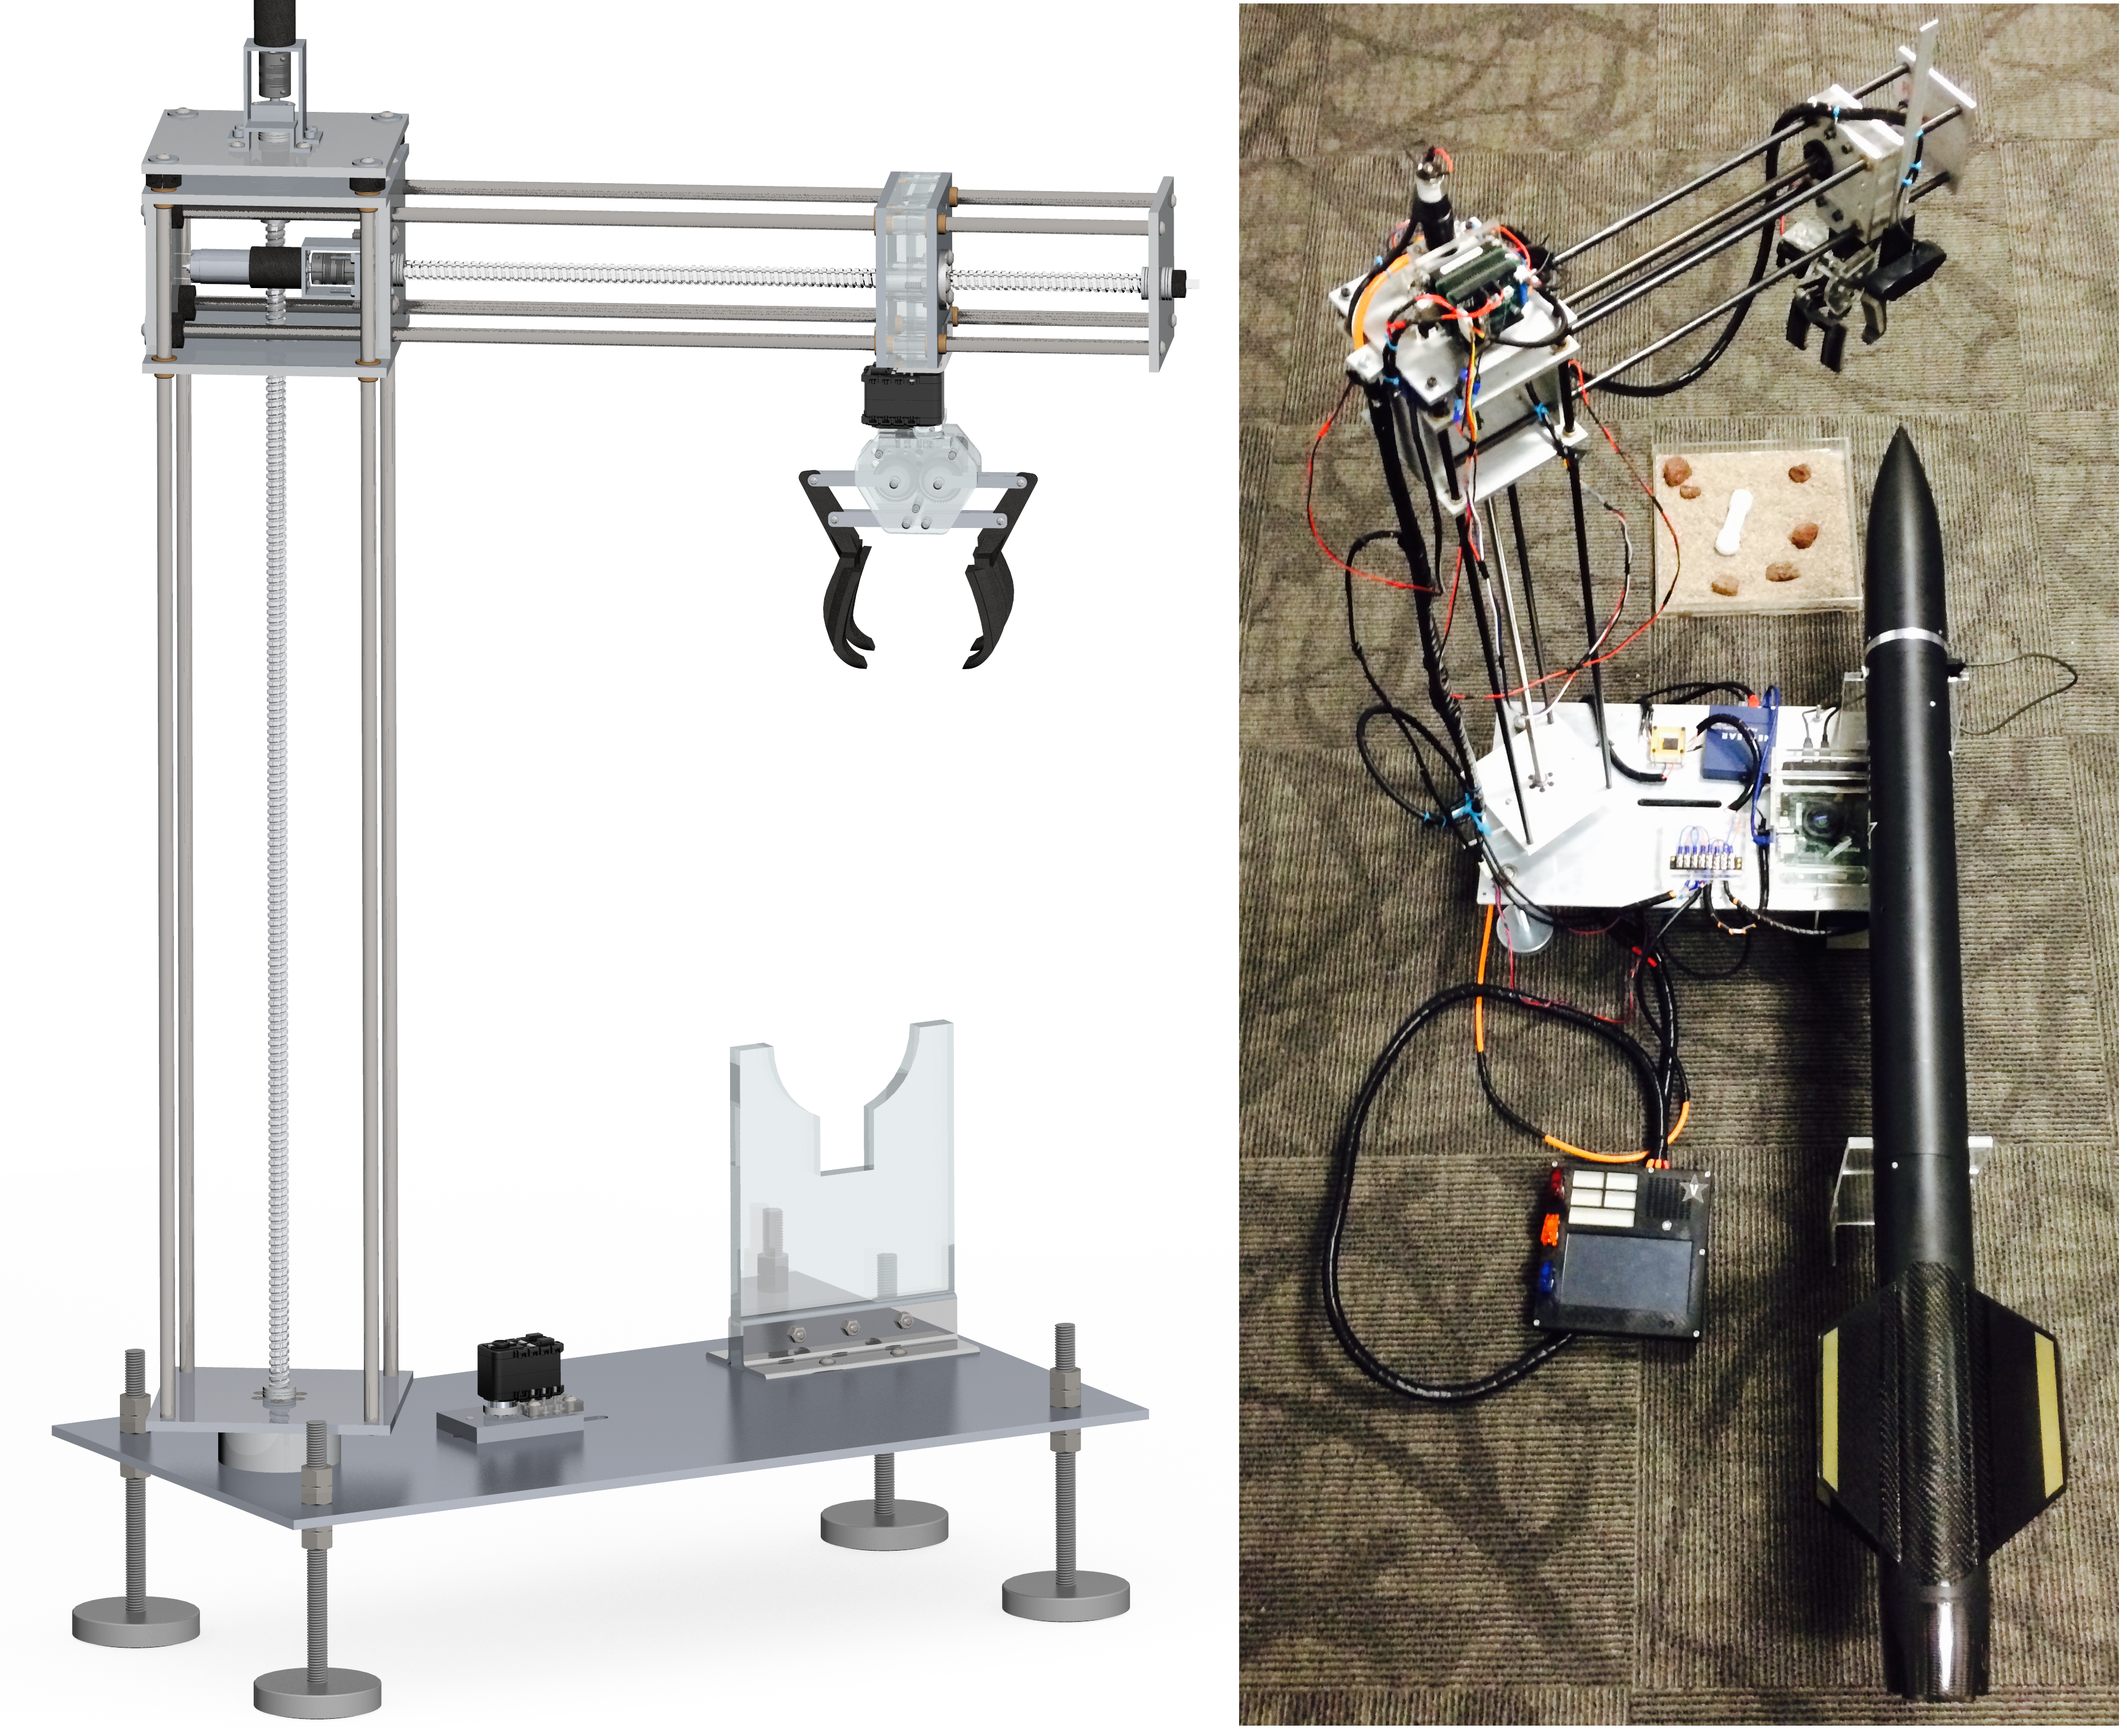
\includegraphics[width=\textwidth]{AGSE_Render.png}
	\caption{AGSE and rocket used in the 2014-2015 NASA SLI
		competition.  The UIP is shown in the bottom left of the
		picture, the Motor Control Board is on the top of the arm of
		the AGSE, and the NVIDIA Jetson is under the rocket.}
	\label{fig:competition_AGSE}
\end{figure}
\FloatBarrier

\subsubsection{Performance Assessment}

At the competition, the Vanderbilt AGSE was able to complete the
sample retrieval process in approximately $4.5$ minutes. The recovery
process, as shown in Figure \ref{fig:AGSE_Operation}, was successful,
with payload and rocket bay recognition occurring quickly and
efficiently. The AGSE was able to grasp the payload using only two of
its four padded end effector phalanges, and successfully deposited the
payload within the rocket bay. This operation received high marks from
the NASA officials and earned the competition's \emph{Autonomous
	Ground Support Equipment Award}.

\begin{figure}[t]
	\centering
	\includegraphics[width=\linewidth]{AGSE_Operation.png}
	\caption{AGSE Calibration and Testing}
	\label{fig:AGSE_Operation}	
\end{figure}
\FloatBarrier

System robustness was validated on the day of competition when a key
component failed and was able to be quickly replaced with a different
part with no detriment to system performance. The Dynamixel AX-12A
servo controlling the base rotational degree of freedom of the AGSE
suffered an irreparable failure of its gearbox and had to be removed
from the robot. A backup of the servo was not readily available, and a
different model servo by the same company had to be swapped in
instead.  This new model, a Dynamixel MX-28T, while having similar
performance as the old servo, had a different communication protocol
and mounting footprint, as well as a more complex control scheme.

The component-based nature of ROSMOD allowed quick modifications of
the business logic of the \emph{rotation\_controller} component to
update the system to use the new hardware.  The new control scheme was
quickly implemented and the control software was updated to account
for the new physical placement of the servo due to its different
mounting footprint. After these modifications were made, the AGSE was
able to perform at its optimal level during its part of the
competition.

\fi



\bibliographystyle{abbrv}
\begin{spacing}{1}
  \bibliography{00-Dissertation}
\end{spacing}
	
\end{document}
